% Build: cd paper && uv run python derive.py && tectonic main.tex
\documentclass[11pt]{article}
\usepackage[margin=1in]{geometry}
\usepackage[T1]{fontenc}
\usepackage{lmodern}
\usepackage{microtype}
\usepackage{amsmath,amssymb}
\usepackage{graphicx}
\usepackage{booktabs}
\usepackage{tikz}
\usepackage[numbers,sort&compress]{natbib}
\usepackage[colorlinks=true,linkcolor=blue,citecolor=blue,urlcolor=blue]{hyperref}
\usepackage{caption}
\captionsetup{font=small,labelfont=bf}
% generated by paper/derive.py; do not edit
\newcommand{\nEmbNormSpread}{1.4e-07}
\newcommand{\nHeads}{25}
\newcommand{\nHidden}{1{,}681}
\newcommand{\nInter}{1{,}860}
\newcommand{\nKdim}{20}
\newcommand{\nLayers}{6}
\newcommand{\nNonzero}{1{,}880{,}041}
\newcommand{\nNonzeroPct}{0.86}
\newcommand{\nParams}{219{,}692{,}711}
\newcommand{\nParamsM}{219.7}
\newcommand{\nPoneOneGate}{1.2e-7}  % PROGRESS.md P1: a one-gate probe measured 1.2e-7
\newcommand{\nPoneTests}{39}  % PROGRESS.md P1: 39 passed
\newcommand{\nPthreeClearTok}{831}
\newcommand{\nPthreeGap}{29.983}
\newcommand{\nPthreeLaptopMs}{135}  % PROGRESS.md P3: about 135 ms per token
\newcommand{\nPthreeLinesTotal}{9}
\newcommand{\nPthreeMultiK}{2}
\newcommand{\nPthreeMultiTok}{832}
\newcommand{\nPthreeRolloutSeconds}{18}  % PROGRESS.md P3: rollout 1873 tokens in 18s
\newcommand{\nPthreeSeed}{10}
\newcommand{\nPthreeTokens}{1{,}873}
\newcommand{\nPtwoBoardFail}{0}
\newcommand{\nPtwoChecked}{7{,}355{,}830}
\newcommand{\nPtwoGames}{10{,}500}
\newcommand{\nPtwoGap}{29.979}
\newcommand{\nPtwoGapMedian}{29.9894}
\newcommand{\nPtwoGreedyBoardFail}{0}
\newcommand{\nPtwoGreedyChecked}{2{,}747{,}880}
\newcommand{\nPtwoGreedyGames}{500}
\newcommand{\nPtwoGreedyGap}{29.9792}
\newcommand{\nPtwoGreedyLines}{18{,}348}
\newcommand{\nPtwoGreedyTokFail}{0}
\newcommand{\nPtwoGreedyTokens}{3{,}629{,}930}
\newcommand{\nPtwoMaxGameTokens}{7{,}849}
\newcommand{\nPtwoRandBoardFail}{0}
\newcommand{\nPtwoRandChecked}{4{,}607{,}950}
\newcommand{\nPtwoRandGames}{10{,}000}
\newcommand{\nPtwoRandGap}{29.9812}
\newcommand{\nPtwoRandLines}{61}
\newcommand{\nPtwoRandTokFail}{0}
\newcommand{\nPtwoRandTokens}{6{,}502{,}442}
\newcommand{\nPtwoResidualErr}{3.22e-06}  % PROGRESS.md P2: compiled: 186 tokens, max residual error 3.22e-06
\newcommand{\nPtwoSeconds}{1518}  % PROGRESS.md P2: RESULT games=10500 failing=0 seconds=1518
\newcommand{\nPtwoTokFail}{0}
\newcommand{\nPtwoTokens}{10{,}132{,}372}
\newcommand{\nPzeroGreedyMulti}{1{,}348}  % PROGRESS.md P0: 18348 lines, 1348 multi-line clears
\newcommand{\nTfVersion}{5.22.1}
\newcommand{\nUnitsA}{1{,}373}
\newcommand{\nUnitsB}{1{,}860}
\newcommand{\nUnitsC}{808}
\newcommand{\nUnitsD}{47}
\newcommand{\nUnitsE}{437}
\newcommand{\nUnitsF}{191}
\newcommand{\nUnitsTotal}{4{,}716}
\newcommand{\nVdim}{45}
\newcommand{\nVocAct}{4}
\newcommand{\nVocLines}{4}
\newcommand{\nVocOther}{4}
\newcommand{\nVocPhase}{5}
\newcommand{\nVocPiece}{7}
\newcommand{\nVocSetp}{14{,}784}
\newcommand{\nVocSrc}{21}
\newcommand{\nVocWrow}{20{,}480}
\newcommand{\nVocab}{35{,}309}
\newcommand{\nVocabParamsM}{118.7}
\newcommand{\nVocabParamsPct}{54}


\newcommand{\tok}[1]{\texttt{#1}}
\newcommand{\silu}{\operatorname{silu}}

\title{Deltris: Tetris Compiled into the Weights of a Stock Qwen3.5 Model}
\author{[author]}
\date{November 2026}

\begin{document}
\maketitle

\begin{abstract}
We compile the rules of Tetris into the weights of an unmodified \texttt{Qwen3\_5ForCausalLM} checkpoint, with no training. The model has \nLayers{} Gated DeltaNet layers and \nParamsM{} million parameters, and it loads with the stock \texttt{transformers} class. Its recurrent state holds the board, one DeltaNet head per row, plus a display head whose state matrix is the whole board. The game runs as a token protocol in which every token the model emits is a write to that memory. Exactness rests on two properties of the construction: every residual coordinate except one padding dimension is exactly 0 or 1, and the residual norm is the same on every token, so each RMSNorm reduces to a known constant. On top of that, a few fp32 identities hold exactly, among them $\silu(30)/30 = 1$, $\sigma(30) = 1$ and a decay of exactly 1. In a differential test against a reference interpreter on \nPtwoGames{} seeded games (\nPtwoTokens{} tokens, of which \nPtwoChecked{} are model-emitted), we observe zero token mismatches and zero mismatches between the board decoded from the recurrent state and the reference board. The smallest logit gap between the correct token and the runner-up is \nPtwoGap{} against a design value of 30. These are observations from one run in fp32 on one GPU, on games of at most \nPtwoMaxGameTokens{} tokens. Long-run stability, reduced precision and the interpretability experiments the model was built for are not yet tested.
\end{abstract}

\section{Introduction}

A network whose weights were written by hand, rather than learned, has a known meaning for every parameter. That makes it a test object for methods that claim to read or repair networks: the reading can be graded against the construction instead of against behaviour alone. Compiled transformers have been used this way since RASP and Tracr~\cite{weiss2021thinking,lindner2023tracr}. Deltris applies the idea to a current production architecture whose sequence mixer is a recurrent layer, Gated DeltaNet~\cite{yang2024gated}, as implemented for Qwen3.5 in \texttt{transformers} \nTfVersion{}.

Gated DeltaNet keeps a matrix-valued state per head and updates it with the delta rule~\cite{schlag2021linear,yang2024parallelizing}. With the gates pinned, the update is an exact overwrite of one row of the state, which turns each head into an addressable memory. Qwenputer~\cite{qwenputer} used this to compile a CPU into Qwen3.5-4B, with DeltaNet state as RAM. Deltris does not emulate a processor. It compiles the game's own rules as a circuit, so the network contains no instruction set and no program counter, and its state matrix, plotted, is the board.

The contributions are these:
\begin{itemize}
\item A compiler from a small circuit description to the weights of a stock \texttt{Qwen3\_5ForCausalLM}, with memory heads in the first DeltaNet layer and Boolean logic in the SwiGLU MLPs (Section~\ref{sec:method}).
\item A set of conditions under which that circuit is exact in fp32: binary residual values, a constant residual norm, and gate and decay values that round to exactly 1 (Section~\ref{sec:exact}).
\item A token protocol for Tetris in which each model-emitted token is one memory write, held to the information the model can see (Section~\ref{sec:protocol}).
\item A differential test on \nPtwoGames{} games with no token or board mismatch, and a free-running game with a two-line clear decoded entirely from the recurrent state (Section~\ref{sec:results}).
\end{itemize}

\section{Background: the Qwen3.5 decoder layer}
\label{sec:background}

We take the architecture from \texttt{modeling\_qwen3\_5.py} in \texttt{transformers} \nTfVersion{}; the facts below are each checked by a test in the repository (\texttt{tests/test\_arch\_facts.py}). A decoder layer computes
\begin{equation}
h \leftarrow h + \mathrm{Mixer}(\mathrm{RMSNorm}(h)), \qquad h \leftarrow h + \mathrm{MLP}(\mathrm{RMSNorm}(h)),
\end{equation}
with $\mathrm{RMSNorm}(x) = x \,/\sqrt{\overline{x^2} + \epsilon}\,\cdot (1 + w)$ and the SwiGLU MLP~\cite{shazeer2020glu} $\mathrm{MLP}(x) = W_d\,(\silu(W_g x) \odot W_u x)$, where $\silu(u) = u\,\sigma(u)$~\cite{elfwing2017silu}. No projection in the MLP or the mixer has a bias.

When the layer type is \texttt{linear\_attention}, the mixer is Gated DeltaNet. Per token, $W_{qkv} x$ passes through a depthwise causal convolution of width 4, then SiLU, and is split into $q$, $k$ and $v$ for each head. The scalars $\beta = \sigma(w_b^\top x)$ and $g = -e^{A}\,\mathrm{softplus}(w_a^\top x + b_{dt})$ set the write strength and the decay. After $q$ and $k$ are L2-normalised and $q$ is divided by $\sqrt{d_k}$, each head with state $S \in \mathbb{R}^{d_k \times d_v}$ computes
\begin{equation}
S \leftarrow e^{g} S, \qquad S \leftarrow S + \beta\, k \,(v - S^\top k)^\top, \qquad o = S^\top q .
\label{eq:delta}
\end{equation}
The head output is $\mathrm{RMSNorm}(o) \odot w \odot \silu(z)$ with $z = W_z x$, followed by an output projection. Run token by token with a cache, this is the recurrent path; the chunked prefill path uses triangular solves and is not used here.

\section{Method}
\label{sec:method}

\subsection{Exactness in fp32}
\label{sec:exact}

Every residual coordinate except one padding dimension, FILL, holds exactly 0 or 1 on every token. A field is either one-hot over its labels or dual-rail (each bit stored as a pair $(b, 1-b)$). A constant coordinate ONE stands in for every bias, since the architecture has none. On binary inputs, five fp32 facts make the circuit exact:
\begin{itemize}
\item $\sigma(30)$ rounds to 1.0, so a write logit of $+30$ gives $\beta = 1$; a logit of $-30$ gives $\beta < 10^{-12}$.
\item With $A = -40$, $e^{A} \approx 4\times 10^{-18}$, and the decay $e^{g}$ is exactly 1.0. The decay input $w_a$ is zero; the per-head $b_{dt}$ enters through a softplus and has no effect at this scale.
\item The convolution kernel is $[0, 0, 0, 1]$, so only the current token reaches $q$, $k$ and $v$, and these are driven to $\{0, 30\}$, where $\silu(30) = 30$ and $\silu(0) = 0$ in fp32.
\item A one-hot vector $30\,e_i$ L2-normalises to exactly $e_i$.
\item $\silu(30)/30 = 1.0$ exactly, and $|\silu(-30)| < 10^{-11}$.
\end{itemize}
Under these values, a write with key $e_s$ and value $v$ in Equation~\ref{eq:delta} sets row $s$ of $S$ to $v$ and leaves every other row unchanged, and a query $e_r$ reads row $r$ back.

The fifth condition is the constant-norm rule. Every embedding row is padded on FILL to the same L2 norm, and every value any layer writes into the residual goes into fresh dimensions whose number of active entries is fixed. The squared residual norm after each sublayer is therefore a constant known to the compiler, the same on every token (\texttt{Program.norm2\_at} in \texttt{deltris/compiler/graph.py}). RMSNorm weights are left at 0, so each RMSNorm multiplies by a known scalar, which the compiler folds into the next projection. The same reasoning covers the gated norm on memory reads: every stored value has a fixed count of active entries, so the per-head normalisation of a read is also a known constant. Reading a slot that was never written returns zero and would break this rule, so the protocol writes every slot before reading it.

\subsection{MLP primitives}

With $G = 30$ and binary $s$ and $x$, one SwiGLU unit with gate weight $G$ on $s$ and up weight $1/G$ on $x$ outputs
\begin{equation}
\silu(G s)\,\frac{x}{G} = s \wedge x ,
\end{equation}
exactly. This gated copy gives a multiplexer bit, a two-input AND, and one row of a lookup table (the gate sums the selected one-hot labels of the inputs, offset on ONE so that only the matching combination reaches $G$). A threshold on an integer sum $u$ of binary terms takes two units,
\begin{equation}
\frac{\silu(G(u - t + 1)) - \silu(G(u - t))}{G} = [u \ge t],
\end{equation}
which gives AND and OR over many inputs, counting, and rule tables. NOT and bijective relabelings are free: they are a different reading of dimensions that already exist (a dual-rail field's off-rail is its negation). The primitives live in \texttt{deltris/compiler/primitives.py}; each registers a NumPy reference function, and the compiler checks the compiled model against the composed references.

\subsection{Memory}

All memory heads live in the mixer of layer 0, where every write is a function of the current token alone. For a head with slots $0, \dots, n-1$, the token's embedding carries a one-hot slot field and a value field. The compiler sets $W_{qkv}$ so that $k = 30\,e_s$ for the slot named by the token and $v = 30 \times$ the value, and sets $w_b$ to $+60$ on the slot field and $-30$ on ONE, so the write logit is $+30$ when the token names a slot and $-30$ otherwise. The query is fixed per head ($30\,e_r$ on ONE), so the head reads slot $r$ after the write on every token. The mixers of layers 1 to 5 have a zero output projection.

Deltris uses \nHeads{} heads with $d_k = \nKdim$ and $d_v = \nVdim$:
\begin{itemize}
\item twenty board heads $B_0, \dots, B_{19}$, where $B_i$ holds board row $i$ as a dual-rail 10-cell value and is always read, so the whole board reaches the residual on every token;
\item a DISPLAY head with 20 slots, written at slot $r$ by every row write and never read (its output projection is zero), whose $20 \times \nVdim$ state matrix is the board;
\item four single-slot registers: PIECE (one-hot type, rotation, $x$ and $y$; 7 + 4 + 12 + 22 = \nVdim{} dimensions, which sets $d_v$), PHASE, and two row pointers T and S used by line clearing.
\end{itemize}

\subsection{Token protocol}
\label{sec:protocol}

The game is a sequence of tokens. The host sends \tok{BOS}, one of \nVocPiece{} \tok{PIECE} tokens when a new piece is needed, and one of \nVocAct{} actions (\tok{LEFT}, \tok{RIGHT}, \tok{ROT\_CW}, \tok{NOOP}) per gravity tick. Every other token is emitted by the model, fed back as the next input, and each one writes memory: \tok{WROW}$(r, \mathit{bits})$ writes board row $r$ (\nVocWrow{} tokens), \tok{SETP}$(\mathit{type}, \mathit{rot}, x, y, \mathit{lock})$ writes PIECE (\nVocSetp{}), \tok{SRC}$(s)$ writes S (\nVocSrc{}) and \tok{PHASE}$(p)$ writes PHASE (\nVocPhase{}). Control tokens (\tok{TICK\_END}, \tok{NEED\_PIECE}, \tok{GAME\_OVER} and \nVocLines{} \tok{LINES}$(k)$ tokens) write nothing. The vocabulary has \nVocab{} tokens. The host loop appends a host token and lets the model generate until it emits \tok{TICK\_END}, \tok{NEED\_PIECE} or \tok{GAME\_OVER}.

A reference interpreter (\texttt{deltris/ref/isa.py}) defines the protocol, and it is held to the model's information limit: its next-token function sees only the current token and the memory after that token's write, never the trace history. An interpreter allowed to see more could define a protocol that no model with this memory can run. Enforcing the limit exposed four gaps in the first protocol design, each recorded in the repository's decision log (\texttt{DECISIONS.md}, D2 to D5):
\begin{itemize}
\item \tok{BOS} writes the whole initial memory in one token, since head $B_i$ is only ever read at its own slot.
\item \tok{SETP} carries a lock bit, so that a piece that locks after a legal move is stored at its post-move position.
\item The entry to the lock and clear phases resets T.
\item \tok{LINES}$(k)$ is emitted at the start of a clear, while the post-lock board still shows which rows are full.
\end{itemize}

A tick in play is \tok{ACT} $\to$ \tok{SETP} $\to$ \tok{TICK\_END}. When the piece locks, the model writes each row the piece occupies, then either spawns the next piece or clears lines: \tok{PHASE(CLEAR)} $\to$ \tok{LINES}$(k)$, then for each target row $t = 19, \dots, 0$ a \tok{SRC} token naming the next non-full source row and a \tok{WROW}$(t, \cdot)$ copying it, then \tok{PHASE(SPAWN)} $\to$ \tok{NEED\_PIECE}. A clear therefore rewrites the board one row per two tokens.

\subsection{The Tetris circuit}

\texttt{compile\_deltris()} (\texttt{deltris/build.py}) expresses the next-token function of the interpreter as a circuit over the token fields and the memory reads, and schedules each primitive in the earliest MLP whose inputs are ready. The longest path sets the depth. It is the action path: read the piece, form the candidate rotation and $x$, look up the candidate's cell mask, AND the mask with the board rows it covers, OR the collisions, choose the new position and the lock bit, and select the output token's fields. That chain needs six MLPs, so the model has \nLayers{} layers; every other path fits inside them. The output fields drive a one-hot LM head with a logit of 30 on the correct token, and decoding is greedy.

Table~\ref{tab:model} lists the compiled sizes. The compiler chose them; none was tuned. More than half of the parameters (\nVocabParamsM{} million, \nVocabParamsPct\%) are the embedding and the LM head over the \nVocab-token vocabulary, and \nNonzeroPct\% of all weights are nonzero.

\begin{table}[t]
\centering
\caption{Compiled model. Source: \texttt{models/deltris/config.json} and \texttt{model.safetensors}, read by \texttt{paper/derive.py}. MLP units are rows of \texttt{gate\_proj} with any nonzero weight.}
\label{tab:model}
\begin{tabular}{lr}
\toprule
hidden size & \nHidden \\
layers (all \texttt{linear\_attention}) & \nLayers \\
DeltaNet heads, $d_k$, $d_v$ & \nHeads, \nKdim, \nVdim \\
intermediate size & \nInter \\
MLP units used, layers 0--5 & \nUnitsA, \nUnitsB, \nUnitsC, \nUnitsD, \nUnitsE, \nUnitsF \\
vocabulary & \nVocab \\
parameters & \nParams \\
nonzero parameters & \nNonzero{} (\nNonzeroPct\%) \\
\bottomrule
\end{tabular}
\end{table}

The compiler writes a configuration and a state dict and saves them with \texttt{save\_pretrained}; \texttt{AutoModelForCausalLM.from\_pretrained} returns a \texttt{Qwen3\_5ForCausalLM} with every tensor bit-identical. One runtime detail is not covered by the stock code path. On \texttt{transformers} \nTfVersion{}, a model whose layers are all \texttt{linear\_attention} raises in the cache's sequence-length query on a cached forward unless the caller passes \texttt{position\_ids} and an attention mask given as a dictionary keyed by layer type; our runner passes both.

\section{Setup}
\label{sec:setup}

\paragraph{Reference.} \texttt{deltris/ref/tetris.py} implements the rules: a $10 \times 20$ board with row 0 at the top, seven pieces with fixed rotation bitmaps and no wall kicks, one action then gravity per tick, and a host-supplied piece sequence from a seeded 7-bag. \texttt{isa.py} implements the protocol. A test suite checks that the two agree after every tick on 10{,}000 random-action games and 500 games of 100 pieces played by a greedy placement policy, together with forced cases (a four-line clear, non-contiguous clears, top-out, a rotation rejected at a wall, a lock after a legal slide). Random play clears few lines (\nPtwoRandLines{} over 10{,}000 games), which is why the greedy set exists: it yields \nPtwoGreedyLines{} lines including \nPzeroGreedyMulti{} multi-line clears.

\paragraph{Primitive tests.} Each primitive is compiled alone into a stock model and run token by token with a cache. The tests cover all inputs of a 6-bit field for the logic primitives, every (type, rotation, $x$) for the lookup tables, 300 random multiplexer selections, a 421-token sequence of memory writes and reads (400 of them random), and $10^6$ alternating writes to one slot fed through the stock recurrent kernel. Every test asserts a margin of at least 0.4 and a residual norm constant to $10^{-5}$ relative at every layer; \nPoneTests{} tests pass.

\paragraph{Differential test.} The compiled model runs the same \nPtwoRandGames{} random and \nPtwoGreedyGames{} greedy games, with the same seeds. The interpreter's trace is fed in token by token, and at every position where the model must emit, the argmax is compared with the interpreter's token. After every token the board is decoded from the DISPLAY head's state (\texttt{cache.get\_recurrent\_state}) and compared with the reference board. If every check passes, the model's own greedy rollout is the fed trace, so the fed test is equal to a free run; it lets games share one batched forward pass. The test ran as one job on an NVIDIA GB10 in fp32 with TF32 disabled for matrix multiplication and cuDNN, with PyTorch 2.15.0 and \texttt{transformers} \nTfVersion{}, and took \nPtwoSeconds{} seconds. The optional \texttt{fla} and \texttt{causal\_conv1d} kernels were absent, so the pure-PyTorch delta rule and convolution ran. Per-game results are in \texttt{results/p2-games.jsonl}.

\paragraph{Free play.} The host loop runs the model with no reference in the loop: the host sends pieces from a seeded 7-bag and actions from a greedy planner that reads only the board and piece decoded from the recurrent state, and the model emits everything else. A recorder draws each frame from the decoded state alone. The rollout used for the figures (seed \nPthreeSeed{}, \nPthreeTokens{} tokens) is in \texttt{results/deltris-p3.pkl}.

\section{Results}
\label{sec:results}

\begin{table}[t]
\centering
\caption{Differential test against the reference interpreter. Source: \texttt{results/p2-games.jsonl}, aggregated by \texttt{paper/derive.py}. ``Checked'' counts model-emitted tokens compared with the reference; the gap is the smallest logit difference between the correct token and the next-best token over all checked positions.}
\label{tab:diff}
\begin{tabular}{lrrrrrrr}
\toprule
games & n & tokens & checked & lines & token fail & board fail & min gap \\
\midrule
random & \nPtwoRandGames & \nPtwoRandTokens & \nPtwoRandChecked & \nPtwoRandLines & \nPtwoRandTokFail & \nPtwoRandBoardFail & \nPtwoRandGap \\
greedy & \nPtwoGreedyGames & \nPtwoGreedyTokens & \nPtwoGreedyChecked & \nPtwoGreedyLines & \nPtwoGreedyTokFail & \nPtwoGreedyBoardFail & \nPtwoGreedyGap \\
\midrule
total & \nPtwoGames & \nPtwoTokens & \nPtwoChecked & & \nPtwoTokFail & \nPtwoBoardFail & \nPtwoGap \\
\bottomrule
\end{tabular}
\end{table}

Table~\ref{tab:diff} gives the differential test. In this run we observe no token mismatch over \nPtwoChecked{} model-emitted tokens and no board mismatch after any of \nPtwoTokens{} tokens. The line totals equal the reference's for the same seeds. The longest game has \nPtwoMaxGameTokens{} tokens.

\begin{figure}[t]
\centering
% generated by paper/derive.py from results/p2-games.jsonl; do not edit
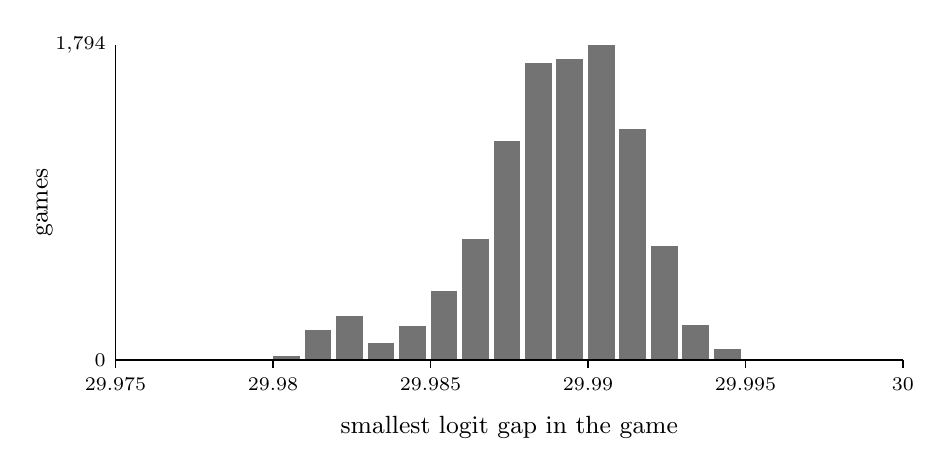
\begin{tikzpicture}
\fill[black!55] (0.000,0) rectangle +(0.340,0.000);
\fill[black!55] (0.400,0) rectangle +(0.340,0.000);
\fill[black!55] (0.800,0) rectangle +(0.340,0.000);
\fill[black!55] (1.200,0) rectangle +(0.340,0.000);
\fill[black!55] (1.600,0) rectangle +(0.340,0.011);
\fill[black!55] (2.000,0) rectangle +(0.340,0.054);
\fill[black!55] (2.400,0) rectangle +(0.340,0.379);
\fill[black!55] (2.800,0) rectangle +(0.340,0.562);
\fill[black!55] (3.200,0) rectangle +(0.340,0.212);
\fill[black!55] (3.600,0) rectangle +(0.340,0.433);
\fill[black!55] (4.000,0) rectangle +(0.340,0.872);
\fill[black!55] (4.400,0) rectangle +(0.340,1.536);
\fill[black!55] (4.800,0) rectangle +(0.340,2.778);
\fill[black!55] (5.200,0) rectangle +(0.340,3.773);
\fill[black!55] (5.600,0) rectangle +(0.340,3.822);
\fill[black!55] (6.000,0) rectangle +(0.340,4.000);
\fill[black!55] (6.400,0) rectangle +(0.340,2.939);
\fill[black!55] (6.800,0) rectangle +(0.340,1.449);
\fill[black!55] (7.200,0) rectangle +(0.340,0.450);
\fill[black!55] (7.600,0) rectangle +(0.340,0.134);
\fill[black!55] (8.000,0) rectangle +(0.340,0.009);
\fill[black!55] (8.400,0) rectangle +(0.340,0.000);
\fill[black!55] (8.800,0) rectangle +(0.340,0.000);
\fill[black!55] (9.200,0) rectangle +(0.340,0.000);
\fill[black!55] (9.600,0) rectangle +(0.340,0.000);
\draw (0,0) -- (10.0,0);
\draw (0.000,0) -- +(0,-0.1) node[below] {\scriptsize 29.975};
\draw (2.000,0) -- +(0,-0.1) node[below] {\scriptsize 29.98};
\draw (4.000,0) -- +(0,-0.1) node[below] {\scriptsize 29.985};
\draw (6.000,0) -- +(0,-0.1) node[below] {\scriptsize 29.99};
\draw (8.000,0) -- +(0,-0.1) node[below] {\scriptsize 29.995};
\draw (10.000,0) -- +(0,-0.1) node[below] {\scriptsize 30};
\node at (5.0,-0.85) {\small smallest logit gap in the game};
\draw (0,0) -- (0,4.0);
\node[left] at (0,4.0) {\scriptsize 1,794};
\node[left] at (0,0) {\scriptsize 0};
\node[rotate=90] at (-0.9,2.0) {\small games};
\end{tikzpicture}

% generated by paper/derive.py from results/p2-games.jsonl
\caption{Smallest logit gap per game over the \nPtwoGames{} games of the differential test. The design gap is 30; the smallest observed value is \nPtwoGap{} and the median per-game minimum is \nPtwoGapMedian. Greedy decoding needs only a positive gap.}
\label{fig:gaps}
\end{figure}

Figure~\ref{fig:gaps} shows how close the logits stay to the design value. The gap is set by the LM head's scale of 30 on exactly binary output fields, so any deviation measures accumulated floating-point error in the residual. The smallest per-game minimum is \nPtwoGap{}, a loss of about 0.02 logits. On a CPU check inside the same job, the largest residual error over 186 tokens was \nPtwoResidualErr; a one-gate probe in the primitive tests measured \nPoneOneGate. We have not traced the source of the remaining error. One candidate is the normalisation constants the compiler folds into projections, which are rounded to fp32; this is a hypothesis.

\begin{figure}[t]
\centering
% generated by paper/derive.py from results/qwentris-p3.pkl; do not edit
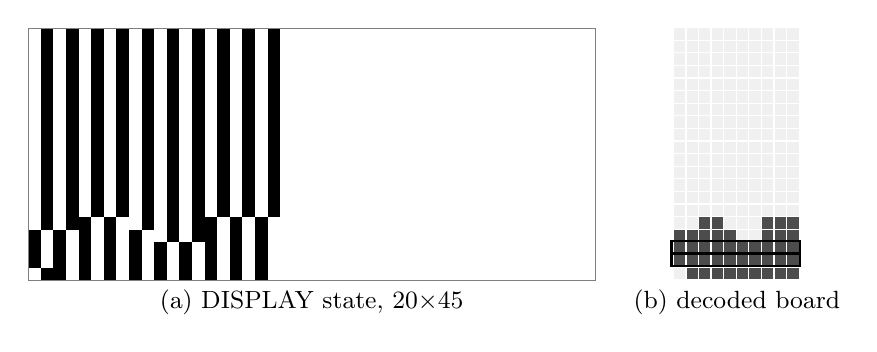
\begin{tikzpicture}
\fill[black!0!white] (0.000,0.000) rectangle +(0.160,-0.160);
\fill[black!100!white] (0.160,0.000) rectangle +(0.160,-0.160);
\fill[black!0!white] (0.320,0.000) rectangle +(0.160,-0.160);
\fill[black!100!white] (0.480,0.000) rectangle +(0.160,-0.160);
\fill[black!0!white] (0.640,0.000) rectangle +(0.160,-0.160);
\fill[black!100!white] (0.800,0.000) rectangle +(0.160,-0.160);
\fill[black!0!white] (0.960,0.000) rectangle +(0.160,-0.160);
\fill[black!100!white] (1.120,0.000) rectangle +(0.160,-0.160);
\fill[black!0!white] (1.280,0.000) rectangle +(0.160,-0.160);
\fill[black!100!white] (1.440,0.000) rectangle +(0.160,-0.160);
\fill[black!0!white] (1.600,0.000) rectangle +(0.160,-0.160);
\fill[black!100!white] (1.760,0.000) rectangle +(0.160,-0.160);
\fill[black!0!white] (1.920,0.000) rectangle +(0.160,-0.160);
\fill[black!100!white] (2.080,0.000) rectangle +(0.160,-0.160);
\fill[black!0!white] (2.240,0.000) rectangle +(0.160,-0.160);
\fill[black!100!white] (2.400,0.000) rectangle +(0.160,-0.160);
\fill[black!0!white] (2.560,0.000) rectangle +(0.160,-0.160);
\fill[black!100!white] (2.720,0.000) rectangle +(0.160,-0.160);
\fill[black!0!white] (2.880,0.000) rectangle +(0.160,-0.160);
\fill[black!100!white] (3.040,0.000) rectangle +(0.160,-0.160);
\fill[black!0!white] (3.200,0.000) rectangle +(0.160,-0.160);
\fill[black!0!white] (3.360,0.000) rectangle +(0.160,-0.160);
\fill[black!0!white] (3.520,0.000) rectangle +(0.160,-0.160);
\fill[black!0!white] (3.680,0.000) rectangle +(0.160,-0.160);
\fill[black!0!white] (3.840,0.000) rectangle +(0.160,-0.160);
\fill[black!0!white] (4.000,0.000) rectangle +(0.160,-0.160);
\fill[black!0!white] (4.160,0.000) rectangle +(0.160,-0.160);
\fill[black!0!white] (4.320,0.000) rectangle +(0.160,-0.160);
\fill[black!0!white] (4.480,0.000) rectangle +(0.160,-0.160);
\fill[black!0!white] (4.640,0.000) rectangle +(0.160,-0.160);
\fill[black!0!white] (4.800,0.000) rectangle +(0.160,-0.160);
\fill[black!0!white] (4.960,0.000) rectangle +(0.160,-0.160);
\fill[black!0!white] (5.120,0.000) rectangle +(0.160,-0.160);
\fill[black!0!white] (5.280,0.000) rectangle +(0.160,-0.160);
\fill[black!0!white] (5.440,0.000) rectangle +(0.160,-0.160);
\fill[black!0!white] (5.600,0.000) rectangle +(0.160,-0.160);
\fill[black!0!white] (5.760,0.000) rectangle +(0.160,-0.160);
\fill[black!0!white] (5.920,0.000) rectangle +(0.160,-0.160);
\fill[black!0!white] (6.080,0.000) rectangle +(0.160,-0.160);
\fill[black!0!white] (6.240,0.000) rectangle +(0.160,-0.160);
\fill[black!0!white] (6.400,0.000) rectangle +(0.160,-0.160);
\fill[black!0!white] (6.560,0.000) rectangle +(0.160,-0.160);
\fill[black!0!white] (6.720,0.000) rectangle +(0.160,-0.160);
\fill[black!0!white] (6.880,0.000) rectangle +(0.160,-0.160);
\fill[black!0!white] (7.040,0.000) rectangle +(0.160,-0.160);
\fill[black!0!white] (0.000,-0.160) rectangle +(0.160,-0.160);
\fill[black!100!white] (0.160,-0.160) rectangle +(0.160,-0.160);
\fill[black!0!white] (0.320,-0.160) rectangle +(0.160,-0.160);
\fill[black!100!white] (0.480,-0.160) rectangle +(0.160,-0.160);
\fill[black!0!white] (0.640,-0.160) rectangle +(0.160,-0.160);
\fill[black!100!white] (0.800,-0.160) rectangle +(0.160,-0.160);
\fill[black!0!white] (0.960,-0.160) rectangle +(0.160,-0.160);
\fill[black!100!white] (1.120,-0.160) rectangle +(0.160,-0.160);
\fill[black!0!white] (1.280,-0.160) rectangle +(0.160,-0.160);
\fill[black!100!white] (1.440,-0.160) rectangle +(0.160,-0.160);
\fill[black!0!white] (1.600,-0.160) rectangle +(0.160,-0.160);
\fill[black!100!white] (1.760,-0.160) rectangle +(0.160,-0.160);
\fill[black!0!white] (1.920,-0.160) rectangle +(0.160,-0.160);
\fill[black!100!white] (2.080,-0.160) rectangle +(0.160,-0.160);
\fill[black!0!white] (2.240,-0.160) rectangle +(0.160,-0.160);
\fill[black!100!white] (2.400,-0.160) rectangle +(0.160,-0.160);
\fill[black!0!white] (2.560,-0.160) rectangle +(0.160,-0.160);
\fill[black!100!white] (2.720,-0.160) rectangle +(0.160,-0.160);
\fill[black!0!white] (2.880,-0.160) rectangle +(0.160,-0.160);
\fill[black!100!white] (3.040,-0.160) rectangle +(0.160,-0.160);
\fill[black!0!white] (3.200,-0.160) rectangle +(0.160,-0.160);
\fill[black!0!white] (3.360,-0.160) rectangle +(0.160,-0.160);
\fill[black!0!white] (3.520,-0.160) rectangle +(0.160,-0.160);
\fill[black!0!white] (3.680,-0.160) rectangle +(0.160,-0.160);
\fill[black!0!white] (3.840,-0.160) rectangle +(0.160,-0.160);
\fill[black!0!white] (4.000,-0.160) rectangle +(0.160,-0.160);
\fill[black!0!white] (4.160,-0.160) rectangle +(0.160,-0.160);
\fill[black!0!white] (4.320,-0.160) rectangle +(0.160,-0.160);
\fill[black!0!white] (4.480,-0.160) rectangle +(0.160,-0.160);
\fill[black!0!white] (4.640,-0.160) rectangle +(0.160,-0.160);
\fill[black!0!white] (4.800,-0.160) rectangle +(0.160,-0.160);
\fill[black!0!white] (4.960,-0.160) rectangle +(0.160,-0.160);
\fill[black!0!white] (5.120,-0.160) rectangle +(0.160,-0.160);
\fill[black!0!white] (5.280,-0.160) rectangle +(0.160,-0.160);
\fill[black!0!white] (5.440,-0.160) rectangle +(0.160,-0.160);
\fill[black!0!white] (5.600,-0.160) rectangle +(0.160,-0.160);
\fill[black!0!white] (5.760,-0.160) rectangle +(0.160,-0.160);
\fill[black!0!white] (5.920,-0.160) rectangle +(0.160,-0.160);
\fill[black!0!white] (6.080,-0.160) rectangle +(0.160,-0.160);
\fill[black!0!white] (6.240,-0.160) rectangle +(0.160,-0.160);
\fill[black!0!white] (6.400,-0.160) rectangle +(0.160,-0.160);
\fill[black!0!white] (6.560,-0.160) rectangle +(0.160,-0.160);
\fill[black!0!white] (6.720,-0.160) rectangle +(0.160,-0.160);
\fill[black!0!white] (6.880,-0.160) rectangle +(0.160,-0.160);
\fill[black!0!white] (7.040,-0.160) rectangle +(0.160,-0.160);
\fill[black!0!white] (0.000,-0.320) rectangle +(0.160,-0.160);
\fill[black!100!white] (0.160,-0.320) rectangle +(0.160,-0.160);
\fill[black!0!white] (0.320,-0.320) rectangle +(0.160,-0.160);
\fill[black!100!white] (0.480,-0.320) rectangle +(0.160,-0.160);
\fill[black!0!white] (0.640,-0.320) rectangle +(0.160,-0.160);
\fill[black!100!white] (0.800,-0.320) rectangle +(0.160,-0.160);
\fill[black!0!white] (0.960,-0.320) rectangle +(0.160,-0.160);
\fill[black!100!white] (1.120,-0.320) rectangle +(0.160,-0.160);
\fill[black!0!white] (1.280,-0.320) rectangle +(0.160,-0.160);
\fill[black!100!white] (1.440,-0.320) rectangle +(0.160,-0.160);
\fill[black!0!white] (1.600,-0.320) rectangle +(0.160,-0.160);
\fill[black!100!white] (1.760,-0.320) rectangle +(0.160,-0.160);
\fill[black!0!white] (1.920,-0.320) rectangle +(0.160,-0.160);
\fill[black!100!white] (2.080,-0.320) rectangle +(0.160,-0.160);
\fill[black!0!white] (2.240,-0.320) rectangle +(0.160,-0.160);
\fill[black!100!white] (2.400,-0.320) rectangle +(0.160,-0.160);
\fill[black!0!white] (2.560,-0.320) rectangle +(0.160,-0.160);
\fill[black!100!white] (2.720,-0.320) rectangle +(0.160,-0.160);
\fill[black!0!white] (2.880,-0.320) rectangle +(0.160,-0.160);
\fill[black!100!white] (3.040,-0.320) rectangle +(0.160,-0.160);
\fill[black!0!white] (3.200,-0.320) rectangle +(0.160,-0.160);
\fill[black!0!white] (3.360,-0.320) rectangle +(0.160,-0.160);
\fill[black!0!white] (3.520,-0.320) rectangle +(0.160,-0.160);
\fill[black!0!white] (3.680,-0.320) rectangle +(0.160,-0.160);
\fill[black!0!white] (3.840,-0.320) rectangle +(0.160,-0.160);
\fill[black!0!white] (4.000,-0.320) rectangle +(0.160,-0.160);
\fill[black!0!white] (4.160,-0.320) rectangle +(0.160,-0.160);
\fill[black!0!white] (4.320,-0.320) rectangle +(0.160,-0.160);
\fill[black!0!white] (4.480,-0.320) rectangle +(0.160,-0.160);
\fill[black!0!white] (4.640,-0.320) rectangle +(0.160,-0.160);
\fill[black!0!white] (4.800,-0.320) rectangle +(0.160,-0.160);
\fill[black!0!white] (4.960,-0.320) rectangle +(0.160,-0.160);
\fill[black!0!white] (5.120,-0.320) rectangle +(0.160,-0.160);
\fill[black!0!white] (5.280,-0.320) rectangle +(0.160,-0.160);
\fill[black!0!white] (5.440,-0.320) rectangle +(0.160,-0.160);
\fill[black!0!white] (5.600,-0.320) rectangle +(0.160,-0.160);
\fill[black!0!white] (5.760,-0.320) rectangle +(0.160,-0.160);
\fill[black!0!white] (5.920,-0.320) rectangle +(0.160,-0.160);
\fill[black!0!white] (6.080,-0.320) rectangle +(0.160,-0.160);
\fill[black!0!white] (6.240,-0.320) rectangle +(0.160,-0.160);
\fill[black!0!white] (6.400,-0.320) rectangle +(0.160,-0.160);
\fill[black!0!white] (6.560,-0.320) rectangle +(0.160,-0.160);
\fill[black!0!white] (6.720,-0.320) rectangle +(0.160,-0.160);
\fill[black!0!white] (6.880,-0.320) rectangle +(0.160,-0.160);
\fill[black!0!white] (7.040,-0.320) rectangle +(0.160,-0.160);
\fill[black!0!white] (0.000,-0.480) rectangle +(0.160,-0.160);
\fill[black!100!white] (0.160,-0.480) rectangle +(0.160,-0.160);
\fill[black!0!white] (0.320,-0.480) rectangle +(0.160,-0.160);
\fill[black!100!white] (0.480,-0.480) rectangle +(0.160,-0.160);
\fill[black!0!white] (0.640,-0.480) rectangle +(0.160,-0.160);
\fill[black!100!white] (0.800,-0.480) rectangle +(0.160,-0.160);
\fill[black!0!white] (0.960,-0.480) rectangle +(0.160,-0.160);
\fill[black!100!white] (1.120,-0.480) rectangle +(0.160,-0.160);
\fill[black!0!white] (1.280,-0.480) rectangle +(0.160,-0.160);
\fill[black!100!white] (1.440,-0.480) rectangle +(0.160,-0.160);
\fill[black!0!white] (1.600,-0.480) rectangle +(0.160,-0.160);
\fill[black!100!white] (1.760,-0.480) rectangle +(0.160,-0.160);
\fill[black!0!white] (1.920,-0.480) rectangle +(0.160,-0.160);
\fill[black!100!white] (2.080,-0.480) rectangle +(0.160,-0.160);
\fill[black!0!white] (2.240,-0.480) rectangle +(0.160,-0.160);
\fill[black!100!white] (2.400,-0.480) rectangle +(0.160,-0.160);
\fill[black!0!white] (2.560,-0.480) rectangle +(0.160,-0.160);
\fill[black!100!white] (2.720,-0.480) rectangle +(0.160,-0.160);
\fill[black!0!white] (2.880,-0.480) rectangle +(0.160,-0.160);
\fill[black!100!white] (3.040,-0.480) rectangle +(0.160,-0.160);
\fill[black!0!white] (3.200,-0.480) rectangle +(0.160,-0.160);
\fill[black!0!white] (3.360,-0.480) rectangle +(0.160,-0.160);
\fill[black!0!white] (3.520,-0.480) rectangle +(0.160,-0.160);
\fill[black!0!white] (3.680,-0.480) rectangle +(0.160,-0.160);
\fill[black!0!white] (3.840,-0.480) rectangle +(0.160,-0.160);
\fill[black!0!white] (4.000,-0.480) rectangle +(0.160,-0.160);
\fill[black!0!white] (4.160,-0.480) rectangle +(0.160,-0.160);
\fill[black!0!white] (4.320,-0.480) rectangle +(0.160,-0.160);
\fill[black!0!white] (4.480,-0.480) rectangle +(0.160,-0.160);
\fill[black!0!white] (4.640,-0.480) rectangle +(0.160,-0.160);
\fill[black!0!white] (4.800,-0.480) rectangle +(0.160,-0.160);
\fill[black!0!white] (4.960,-0.480) rectangle +(0.160,-0.160);
\fill[black!0!white] (5.120,-0.480) rectangle +(0.160,-0.160);
\fill[black!0!white] (5.280,-0.480) rectangle +(0.160,-0.160);
\fill[black!0!white] (5.440,-0.480) rectangle +(0.160,-0.160);
\fill[black!0!white] (5.600,-0.480) rectangle +(0.160,-0.160);
\fill[black!0!white] (5.760,-0.480) rectangle +(0.160,-0.160);
\fill[black!0!white] (5.920,-0.480) rectangle +(0.160,-0.160);
\fill[black!0!white] (6.080,-0.480) rectangle +(0.160,-0.160);
\fill[black!0!white] (6.240,-0.480) rectangle +(0.160,-0.160);
\fill[black!0!white] (6.400,-0.480) rectangle +(0.160,-0.160);
\fill[black!0!white] (6.560,-0.480) rectangle +(0.160,-0.160);
\fill[black!0!white] (6.720,-0.480) rectangle +(0.160,-0.160);
\fill[black!0!white] (6.880,-0.480) rectangle +(0.160,-0.160);
\fill[black!0!white] (7.040,-0.480) rectangle +(0.160,-0.160);
\fill[black!0!white] (0.000,-0.640) rectangle +(0.160,-0.160);
\fill[black!100!white] (0.160,-0.640) rectangle +(0.160,-0.160);
\fill[black!0!white] (0.320,-0.640) rectangle +(0.160,-0.160);
\fill[black!100!white] (0.480,-0.640) rectangle +(0.160,-0.160);
\fill[black!0!white] (0.640,-0.640) rectangle +(0.160,-0.160);
\fill[black!100!white] (0.800,-0.640) rectangle +(0.160,-0.160);
\fill[black!0!white] (0.960,-0.640) rectangle +(0.160,-0.160);
\fill[black!100!white] (1.120,-0.640) rectangle +(0.160,-0.160);
\fill[black!0!white] (1.280,-0.640) rectangle +(0.160,-0.160);
\fill[black!100!white] (1.440,-0.640) rectangle +(0.160,-0.160);
\fill[black!0!white] (1.600,-0.640) rectangle +(0.160,-0.160);
\fill[black!100!white] (1.760,-0.640) rectangle +(0.160,-0.160);
\fill[black!0!white] (1.920,-0.640) rectangle +(0.160,-0.160);
\fill[black!100!white] (2.080,-0.640) rectangle +(0.160,-0.160);
\fill[black!0!white] (2.240,-0.640) rectangle +(0.160,-0.160);
\fill[black!100!white] (2.400,-0.640) rectangle +(0.160,-0.160);
\fill[black!0!white] (2.560,-0.640) rectangle +(0.160,-0.160);
\fill[black!100!white] (2.720,-0.640) rectangle +(0.160,-0.160);
\fill[black!0!white] (2.880,-0.640) rectangle +(0.160,-0.160);
\fill[black!100!white] (3.040,-0.640) rectangle +(0.160,-0.160);
\fill[black!0!white] (3.200,-0.640) rectangle +(0.160,-0.160);
\fill[black!0!white] (3.360,-0.640) rectangle +(0.160,-0.160);
\fill[black!0!white] (3.520,-0.640) rectangle +(0.160,-0.160);
\fill[black!0!white] (3.680,-0.640) rectangle +(0.160,-0.160);
\fill[black!0!white] (3.840,-0.640) rectangle +(0.160,-0.160);
\fill[black!0!white] (4.000,-0.640) rectangle +(0.160,-0.160);
\fill[black!0!white] (4.160,-0.640) rectangle +(0.160,-0.160);
\fill[black!0!white] (4.320,-0.640) rectangle +(0.160,-0.160);
\fill[black!0!white] (4.480,-0.640) rectangle +(0.160,-0.160);
\fill[black!0!white] (4.640,-0.640) rectangle +(0.160,-0.160);
\fill[black!0!white] (4.800,-0.640) rectangle +(0.160,-0.160);
\fill[black!0!white] (4.960,-0.640) rectangle +(0.160,-0.160);
\fill[black!0!white] (5.120,-0.640) rectangle +(0.160,-0.160);
\fill[black!0!white] (5.280,-0.640) rectangle +(0.160,-0.160);
\fill[black!0!white] (5.440,-0.640) rectangle +(0.160,-0.160);
\fill[black!0!white] (5.600,-0.640) rectangle +(0.160,-0.160);
\fill[black!0!white] (5.760,-0.640) rectangle +(0.160,-0.160);
\fill[black!0!white] (5.920,-0.640) rectangle +(0.160,-0.160);
\fill[black!0!white] (6.080,-0.640) rectangle +(0.160,-0.160);
\fill[black!0!white] (6.240,-0.640) rectangle +(0.160,-0.160);
\fill[black!0!white] (6.400,-0.640) rectangle +(0.160,-0.160);
\fill[black!0!white] (6.560,-0.640) rectangle +(0.160,-0.160);
\fill[black!0!white] (6.720,-0.640) rectangle +(0.160,-0.160);
\fill[black!0!white] (6.880,-0.640) rectangle +(0.160,-0.160);
\fill[black!0!white] (7.040,-0.640) rectangle +(0.160,-0.160);
\fill[black!0!white] (0.000,-0.800) rectangle +(0.160,-0.160);
\fill[black!100!white] (0.160,-0.800) rectangle +(0.160,-0.160);
\fill[black!0!white] (0.320,-0.800) rectangle +(0.160,-0.160);
\fill[black!100!white] (0.480,-0.800) rectangle +(0.160,-0.160);
\fill[black!0!white] (0.640,-0.800) rectangle +(0.160,-0.160);
\fill[black!100!white] (0.800,-0.800) rectangle +(0.160,-0.160);
\fill[black!0!white] (0.960,-0.800) rectangle +(0.160,-0.160);
\fill[black!100!white] (1.120,-0.800) rectangle +(0.160,-0.160);
\fill[black!0!white] (1.280,-0.800) rectangle +(0.160,-0.160);
\fill[black!100!white] (1.440,-0.800) rectangle +(0.160,-0.160);
\fill[black!0!white] (1.600,-0.800) rectangle +(0.160,-0.160);
\fill[black!100!white] (1.760,-0.800) rectangle +(0.160,-0.160);
\fill[black!0!white] (1.920,-0.800) rectangle +(0.160,-0.160);
\fill[black!100!white] (2.080,-0.800) rectangle +(0.160,-0.160);
\fill[black!0!white] (2.240,-0.800) rectangle +(0.160,-0.160);
\fill[black!100!white] (2.400,-0.800) rectangle +(0.160,-0.160);
\fill[black!0!white] (2.560,-0.800) rectangle +(0.160,-0.160);
\fill[black!100!white] (2.720,-0.800) rectangle +(0.160,-0.160);
\fill[black!0!white] (2.880,-0.800) rectangle +(0.160,-0.160);
\fill[black!100!white] (3.040,-0.800) rectangle +(0.160,-0.160);
\fill[black!0!white] (3.200,-0.800) rectangle +(0.160,-0.160);
\fill[black!0!white] (3.360,-0.800) rectangle +(0.160,-0.160);
\fill[black!0!white] (3.520,-0.800) rectangle +(0.160,-0.160);
\fill[black!0!white] (3.680,-0.800) rectangle +(0.160,-0.160);
\fill[black!0!white] (3.840,-0.800) rectangle +(0.160,-0.160);
\fill[black!0!white] (4.000,-0.800) rectangle +(0.160,-0.160);
\fill[black!0!white] (4.160,-0.800) rectangle +(0.160,-0.160);
\fill[black!0!white] (4.320,-0.800) rectangle +(0.160,-0.160);
\fill[black!0!white] (4.480,-0.800) rectangle +(0.160,-0.160);
\fill[black!0!white] (4.640,-0.800) rectangle +(0.160,-0.160);
\fill[black!0!white] (4.800,-0.800) rectangle +(0.160,-0.160);
\fill[black!0!white] (4.960,-0.800) rectangle +(0.160,-0.160);
\fill[black!0!white] (5.120,-0.800) rectangle +(0.160,-0.160);
\fill[black!0!white] (5.280,-0.800) rectangle +(0.160,-0.160);
\fill[black!0!white] (5.440,-0.800) rectangle +(0.160,-0.160);
\fill[black!0!white] (5.600,-0.800) rectangle +(0.160,-0.160);
\fill[black!0!white] (5.760,-0.800) rectangle +(0.160,-0.160);
\fill[black!0!white] (5.920,-0.800) rectangle +(0.160,-0.160);
\fill[black!0!white] (6.080,-0.800) rectangle +(0.160,-0.160);
\fill[black!0!white] (6.240,-0.800) rectangle +(0.160,-0.160);
\fill[black!0!white] (6.400,-0.800) rectangle +(0.160,-0.160);
\fill[black!0!white] (6.560,-0.800) rectangle +(0.160,-0.160);
\fill[black!0!white] (6.720,-0.800) rectangle +(0.160,-0.160);
\fill[black!0!white] (6.880,-0.800) rectangle +(0.160,-0.160);
\fill[black!0!white] (7.040,-0.800) rectangle +(0.160,-0.160);
\fill[black!0!white] (0.000,-0.960) rectangle +(0.160,-0.160);
\fill[black!100!white] (0.160,-0.960) rectangle +(0.160,-0.160);
\fill[black!0!white] (0.320,-0.960) rectangle +(0.160,-0.160);
\fill[black!100!white] (0.480,-0.960) rectangle +(0.160,-0.160);
\fill[black!0!white] (0.640,-0.960) rectangle +(0.160,-0.160);
\fill[black!100!white] (0.800,-0.960) rectangle +(0.160,-0.160);
\fill[black!0!white] (0.960,-0.960) rectangle +(0.160,-0.160);
\fill[black!100!white] (1.120,-0.960) rectangle +(0.160,-0.160);
\fill[black!0!white] (1.280,-0.960) rectangle +(0.160,-0.160);
\fill[black!100!white] (1.440,-0.960) rectangle +(0.160,-0.160);
\fill[black!0!white] (1.600,-0.960) rectangle +(0.160,-0.160);
\fill[black!100!white] (1.760,-0.960) rectangle +(0.160,-0.160);
\fill[black!0!white] (1.920,-0.960) rectangle +(0.160,-0.160);
\fill[black!100!white] (2.080,-0.960) rectangle +(0.160,-0.160);
\fill[black!0!white] (2.240,-0.960) rectangle +(0.160,-0.160);
\fill[black!100!white] (2.400,-0.960) rectangle +(0.160,-0.160);
\fill[black!0!white] (2.560,-0.960) rectangle +(0.160,-0.160);
\fill[black!100!white] (2.720,-0.960) rectangle +(0.160,-0.160);
\fill[black!0!white] (2.880,-0.960) rectangle +(0.160,-0.160);
\fill[black!100!white] (3.040,-0.960) rectangle +(0.160,-0.160);
\fill[black!0!white] (3.200,-0.960) rectangle +(0.160,-0.160);
\fill[black!0!white] (3.360,-0.960) rectangle +(0.160,-0.160);
\fill[black!0!white] (3.520,-0.960) rectangle +(0.160,-0.160);
\fill[black!0!white] (3.680,-0.960) rectangle +(0.160,-0.160);
\fill[black!0!white] (3.840,-0.960) rectangle +(0.160,-0.160);
\fill[black!0!white] (4.000,-0.960) rectangle +(0.160,-0.160);
\fill[black!0!white] (4.160,-0.960) rectangle +(0.160,-0.160);
\fill[black!0!white] (4.320,-0.960) rectangle +(0.160,-0.160);
\fill[black!0!white] (4.480,-0.960) rectangle +(0.160,-0.160);
\fill[black!0!white] (4.640,-0.960) rectangle +(0.160,-0.160);
\fill[black!0!white] (4.800,-0.960) rectangle +(0.160,-0.160);
\fill[black!0!white] (4.960,-0.960) rectangle +(0.160,-0.160);
\fill[black!0!white] (5.120,-0.960) rectangle +(0.160,-0.160);
\fill[black!0!white] (5.280,-0.960) rectangle +(0.160,-0.160);
\fill[black!0!white] (5.440,-0.960) rectangle +(0.160,-0.160);
\fill[black!0!white] (5.600,-0.960) rectangle +(0.160,-0.160);
\fill[black!0!white] (5.760,-0.960) rectangle +(0.160,-0.160);
\fill[black!0!white] (5.920,-0.960) rectangle +(0.160,-0.160);
\fill[black!0!white] (6.080,-0.960) rectangle +(0.160,-0.160);
\fill[black!0!white] (6.240,-0.960) rectangle +(0.160,-0.160);
\fill[black!0!white] (6.400,-0.960) rectangle +(0.160,-0.160);
\fill[black!0!white] (6.560,-0.960) rectangle +(0.160,-0.160);
\fill[black!0!white] (6.720,-0.960) rectangle +(0.160,-0.160);
\fill[black!0!white] (6.880,-0.960) rectangle +(0.160,-0.160);
\fill[black!0!white] (7.040,-0.960) rectangle +(0.160,-0.160);
\fill[black!0!white] (0.000,-1.120) rectangle +(0.160,-0.160);
\fill[black!100!white] (0.160,-1.120) rectangle +(0.160,-0.160);
\fill[black!0!white] (0.320,-1.120) rectangle +(0.160,-0.160);
\fill[black!100!white] (0.480,-1.120) rectangle +(0.160,-0.160);
\fill[black!0!white] (0.640,-1.120) rectangle +(0.160,-0.160);
\fill[black!100!white] (0.800,-1.120) rectangle +(0.160,-0.160);
\fill[black!0!white] (0.960,-1.120) rectangle +(0.160,-0.160);
\fill[black!100!white] (1.120,-1.120) rectangle +(0.160,-0.160);
\fill[black!0!white] (1.280,-1.120) rectangle +(0.160,-0.160);
\fill[black!100!white] (1.440,-1.120) rectangle +(0.160,-0.160);
\fill[black!0!white] (1.600,-1.120) rectangle +(0.160,-0.160);
\fill[black!100!white] (1.760,-1.120) rectangle +(0.160,-0.160);
\fill[black!0!white] (1.920,-1.120) rectangle +(0.160,-0.160);
\fill[black!100!white] (2.080,-1.120) rectangle +(0.160,-0.160);
\fill[black!0!white] (2.240,-1.120) rectangle +(0.160,-0.160);
\fill[black!100!white] (2.400,-1.120) rectangle +(0.160,-0.160);
\fill[black!0!white] (2.560,-1.120) rectangle +(0.160,-0.160);
\fill[black!100!white] (2.720,-1.120) rectangle +(0.160,-0.160);
\fill[black!0!white] (2.880,-1.120) rectangle +(0.160,-0.160);
\fill[black!100!white] (3.040,-1.120) rectangle +(0.160,-0.160);
\fill[black!0!white] (3.200,-1.120) rectangle +(0.160,-0.160);
\fill[black!0!white] (3.360,-1.120) rectangle +(0.160,-0.160);
\fill[black!0!white] (3.520,-1.120) rectangle +(0.160,-0.160);
\fill[black!0!white] (3.680,-1.120) rectangle +(0.160,-0.160);
\fill[black!0!white] (3.840,-1.120) rectangle +(0.160,-0.160);
\fill[black!0!white] (4.000,-1.120) rectangle +(0.160,-0.160);
\fill[black!0!white] (4.160,-1.120) rectangle +(0.160,-0.160);
\fill[black!0!white] (4.320,-1.120) rectangle +(0.160,-0.160);
\fill[black!0!white] (4.480,-1.120) rectangle +(0.160,-0.160);
\fill[black!0!white] (4.640,-1.120) rectangle +(0.160,-0.160);
\fill[black!0!white] (4.800,-1.120) rectangle +(0.160,-0.160);
\fill[black!0!white] (4.960,-1.120) rectangle +(0.160,-0.160);
\fill[black!0!white] (5.120,-1.120) rectangle +(0.160,-0.160);
\fill[black!0!white] (5.280,-1.120) rectangle +(0.160,-0.160);
\fill[black!0!white] (5.440,-1.120) rectangle +(0.160,-0.160);
\fill[black!0!white] (5.600,-1.120) rectangle +(0.160,-0.160);
\fill[black!0!white] (5.760,-1.120) rectangle +(0.160,-0.160);
\fill[black!0!white] (5.920,-1.120) rectangle +(0.160,-0.160);
\fill[black!0!white] (6.080,-1.120) rectangle +(0.160,-0.160);
\fill[black!0!white] (6.240,-1.120) rectangle +(0.160,-0.160);
\fill[black!0!white] (6.400,-1.120) rectangle +(0.160,-0.160);
\fill[black!0!white] (6.560,-1.120) rectangle +(0.160,-0.160);
\fill[black!0!white] (6.720,-1.120) rectangle +(0.160,-0.160);
\fill[black!0!white] (6.880,-1.120) rectangle +(0.160,-0.160);
\fill[black!0!white] (7.040,-1.120) rectangle +(0.160,-0.160);
\fill[black!0!white] (0.000,-1.280) rectangle +(0.160,-0.160);
\fill[black!100!white] (0.160,-1.280) rectangle +(0.160,-0.160);
\fill[black!0!white] (0.320,-1.280) rectangle +(0.160,-0.160);
\fill[black!100!white] (0.480,-1.280) rectangle +(0.160,-0.160);
\fill[black!0!white] (0.640,-1.280) rectangle +(0.160,-0.160);
\fill[black!100!white] (0.800,-1.280) rectangle +(0.160,-0.160);
\fill[black!0!white] (0.960,-1.280) rectangle +(0.160,-0.160);
\fill[black!100!white] (1.120,-1.280) rectangle +(0.160,-0.160);
\fill[black!0!white] (1.280,-1.280) rectangle +(0.160,-0.160);
\fill[black!100!white] (1.440,-1.280) rectangle +(0.160,-0.160);
\fill[black!0!white] (1.600,-1.280) rectangle +(0.160,-0.160);
\fill[black!100!white] (1.760,-1.280) rectangle +(0.160,-0.160);
\fill[black!0!white] (1.920,-1.280) rectangle +(0.160,-0.160);
\fill[black!100!white] (2.080,-1.280) rectangle +(0.160,-0.160);
\fill[black!0!white] (2.240,-1.280) rectangle +(0.160,-0.160);
\fill[black!100!white] (2.400,-1.280) rectangle +(0.160,-0.160);
\fill[black!0!white] (2.560,-1.280) rectangle +(0.160,-0.160);
\fill[black!100!white] (2.720,-1.280) rectangle +(0.160,-0.160);
\fill[black!0!white] (2.880,-1.280) rectangle +(0.160,-0.160);
\fill[black!100!white] (3.040,-1.280) rectangle +(0.160,-0.160);
\fill[black!0!white] (3.200,-1.280) rectangle +(0.160,-0.160);
\fill[black!0!white] (3.360,-1.280) rectangle +(0.160,-0.160);
\fill[black!0!white] (3.520,-1.280) rectangle +(0.160,-0.160);
\fill[black!0!white] (3.680,-1.280) rectangle +(0.160,-0.160);
\fill[black!0!white] (3.840,-1.280) rectangle +(0.160,-0.160);
\fill[black!0!white] (4.000,-1.280) rectangle +(0.160,-0.160);
\fill[black!0!white] (4.160,-1.280) rectangle +(0.160,-0.160);
\fill[black!0!white] (4.320,-1.280) rectangle +(0.160,-0.160);
\fill[black!0!white] (4.480,-1.280) rectangle +(0.160,-0.160);
\fill[black!0!white] (4.640,-1.280) rectangle +(0.160,-0.160);
\fill[black!0!white] (4.800,-1.280) rectangle +(0.160,-0.160);
\fill[black!0!white] (4.960,-1.280) rectangle +(0.160,-0.160);
\fill[black!0!white] (5.120,-1.280) rectangle +(0.160,-0.160);
\fill[black!0!white] (5.280,-1.280) rectangle +(0.160,-0.160);
\fill[black!0!white] (5.440,-1.280) rectangle +(0.160,-0.160);
\fill[black!0!white] (5.600,-1.280) rectangle +(0.160,-0.160);
\fill[black!0!white] (5.760,-1.280) rectangle +(0.160,-0.160);
\fill[black!0!white] (5.920,-1.280) rectangle +(0.160,-0.160);
\fill[black!0!white] (6.080,-1.280) rectangle +(0.160,-0.160);
\fill[black!0!white] (6.240,-1.280) rectangle +(0.160,-0.160);
\fill[black!0!white] (6.400,-1.280) rectangle +(0.160,-0.160);
\fill[black!0!white] (6.560,-1.280) rectangle +(0.160,-0.160);
\fill[black!0!white] (6.720,-1.280) rectangle +(0.160,-0.160);
\fill[black!0!white] (6.880,-1.280) rectangle +(0.160,-0.160);
\fill[black!0!white] (7.040,-1.280) rectangle +(0.160,-0.160);
\fill[black!0!white] (0.000,-1.440) rectangle +(0.160,-0.160);
\fill[black!100!white] (0.160,-1.440) rectangle +(0.160,-0.160);
\fill[black!0!white] (0.320,-1.440) rectangle +(0.160,-0.160);
\fill[black!100!white] (0.480,-1.440) rectangle +(0.160,-0.160);
\fill[black!0!white] (0.640,-1.440) rectangle +(0.160,-0.160);
\fill[black!100!white] (0.800,-1.440) rectangle +(0.160,-0.160);
\fill[black!0!white] (0.960,-1.440) rectangle +(0.160,-0.160);
\fill[black!100!white] (1.120,-1.440) rectangle +(0.160,-0.160);
\fill[black!0!white] (1.280,-1.440) rectangle +(0.160,-0.160);
\fill[black!100!white] (1.440,-1.440) rectangle +(0.160,-0.160);
\fill[black!0!white] (1.600,-1.440) rectangle +(0.160,-0.160);
\fill[black!100!white] (1.760,-1.440) rectangle +(0.160,-0.160);
\fill[black!0!white] (1.920,-1.440) rectangle +(0.160,-0.160);
\fill[black!100!white] (2.080,-1.440) rectangle +(0.160,-0.160);
\fill[black!0!white] (2.240,-1.440) rectangle +(0.160,-0.160);
\fill[black!100!white] (2.400,-1.440) rectangle +(0.160,-0.160);
\fill[black!0!white] (2.560,-1.440) rectangle +(0.160,-0.160);
\fill[black!100!white] (2.720,-1.440) rectangle +(0.160,-0.160);
\fill[black!0!white] (2.880,-1.440) rectangle +(0.160,-0.160);
\fill[black!100!white] (3.040,-1.440) rectangle +(0.160,-0.160);
\fill[black!0!white] (3.200,-1.440) rectangle +(0.160,-0.160);
\fill[black!0!white] (3.360,-1.440) rectangle +(0.160,-0.160);
\fill[black!0!white] (3.520,-1.440) rectangle +(0.160,-0.160);
\fill[black!0!white] (3.680,-1.440) rectangle +(0.160,-0.160);
\fill[black!0!white] (3.840,-1.440) rectangle +(0.160,-0.160);
\fill[black!0!white] (4.000,-1.440) rectangle +(0.160,-0.160);
\fill[black!0!white] (4.160,-1.440) rectangle +(0.160,-0.160);
\fill[black!0!white] (4.320,-1.440) rectangle +(0.160,-0.160);
\fill[black!0!white] (4.480,-1.440) rectangle +(0.160,-0.160);
\fill[black!0!white] (4.640,-1.440) rectangle +(0.160,-0.160);
\fill[black!0!white] (4.800,-1.440) rectangle +(0.160,-0.160);
\fill[black!0!white] (4.960,-1.440) rectangle +(0.160,-0.160);
\fill[black!0!white] (5.120,-1.440) rectangle +(0.160,-0.160);
\fill[black!0!white] (5.280,-1.440) rectangle +(0.160,-0.160);
\fill[black!0!white] (5.440,-1.440) rectangle +(0.160,-0.160);
\fill[black!0!white] (5.600,-1.440) rectangle +(0.160,-0.160);
\fill[black!0!white] (5.760,-1.440) rectangle +(0.160,-0.160);
\fill[black!0!white] (5.920,-1.440) rectangle +(0.160,-0.160);
\fill[black!0!white] (6.080,-1.440) rectangle +(0.160,-0.160);
\fill[black!0!white] (6.240,-1.440) rectangle +(0.160,-0.160);
\fill[black!0!white] (6.400,-1.440) rectangle +(0.160,-0.160);
\fill[black!0!white] (6.560,-1.440) rectangle +(0.160,-0.160);
\fill[black!0!white] (6.720,-1.440) rectangle +(0.160,-0.160);
\fill[black!0!white] (6.880,-1.440) rectangle +(0.160,-0.160);
\fill[black!0!white] (7.040,-1.440) rectangle +(0.160,-0.160);
\fill[black!0!white] (0.000,-1.600) rectangle +(0.160,-0.160);
\fill[black!100!white] (0.160,-1.600) rectangle +(0.160,-0.160);
\fill[black!0!white] (0.320,-1.600) rectangle +(0.160,-0.160);
\fill[black!100!white] (0.480,-1.600) rectangle +(0.160,-0.160);
\fill[black!0!white] (0.640,-1.600) rectangle +(0.160,-0.160);
\fill[black!100!white] (0.800,-1.600) rectangle +(0.160,-0.160);
\fill[black!0!white] (0.960,-1.600) rectangle +(0.160,-0.160);
\fill[black!100!white] (1.120,-1.600) rectangle +(0.160,-0.160);
\fill[black!0!white] (1.280,-1.600) rectangle +(0.160,-0.160);
\fill[black!100!white] (1.440,-1.600) rectangle +(0.160,-0.160);
\fill[black!0!white] (1.600,-1.600) rectangle +(0.160,-0.160);
\fill[black!100!white] (1.760,-1.600) rectangle +(0.160,-0.160);
\fill[black!0!white] (1.920,-1.600) rectangle +(0.160,-0.160);
\fill[black!100!white] (2.080,-1.600) rectangle +(0.160,-0.160);
\fill[black!0!white] (2.240,-1.600) rectangle +(0.160,-0.160);
\fill[black!100!white] (2.400,-1.600) rectangle +(0.160,-0.160);
\fill[black!0!white] (2.560,-1.600) rectangle +(0.160,-0.160);
\fill[black!100!white] (2.720,-1.600) rectangle +(0.160,-0.160);
\fill[black!0!white] (2.880,-1.600) rectangle +(0.160,-0.160);
\fill[black!100!white] (3.040,-1.600) rectangle +(0.160,-0.160);
\fill[black!0!white] (3.200,-1.600) rectangle +(0.160,-0.160);
\fill[black!0!white] (3.360,-1.600) rectangle +(0.160,-0.160);
\fill[black!0!white] (3.520,-1.600) rectangle +(0.160,-0.160);
\fill[black!0!white] (3.680,-1.600) rectangle +(0.160,-0.160);
\fill[black!0!white] (3.840,-1.600) rectangle +(0.160,-0.160);
\fill[black!0!white] (4.000,-1.600) rectangle +(0.160,-0.160);
\fill[black!0!white] (4.160,-1.600) rectangle +(0.160,-0.160);
\fill[black!0!white] (4.320,-1.600) rectangle +(0.160,-0.160);
\fill[black!0!white] (4.480,-1.600) rectangle +(0.160,-0.160);
\fill[black!0!white] (4.640,-1.600) rectangle +(0.160,-0.160);
\fill[black!0!white] (4.800,-1.600) rectangle +(0.160,-0.160);
\fill[black!0!white] (4.960,-1.600) rectangle +(0.160,-0.160);
\fill[black!0!white] (5.120,-1.600) rectangle +(0.160,-0.160);
\fill[black!0!white] (5.280,-1.600) rectangle +(0.160,-0.160);
\fill[black!0!white] (5.440,-1.600) rectangle +(0.160,-0.160);
\fill[black!0!white] (5.600,-1.600) rectangle +(0.160,-0.160);
\fill[black!0!white] (5.760,-1.600) rectangle +(0.160,-0.160);
\fill[black!0!white] (5.920,-1.600) rectangle +(0.160,-0.160);
\fill[black!0!white] (6.080,-1.600) rectangle +(0.160,-0.160);
\fill[black!0!white] (6.240,-1.600) rectangle +(0.160,-0.160);
\fill[black!0!white] (6.400,-1.600) rectangle +(0.160,-0.160);
\fill[black!0!white] (6.560,-1.600) rectangle +(0.160,-0.160);
\fill[black!0!white] (6.720,-1.600) rectangle +(0.160,-0.160);
\fill[black!0!white] (6.880,-1.600) rectangle +(0.160,-0.160);
\fill[black!0!white] (7.040,-1.600) rectangle +(0.160,-0.160);
\fill[black!0!white] (0.000,-1.760) rectangle +(0.160,-0.160);
\fill[black!100!white] (0.160,-1.760) rectangle +(0.160,-0.160);
\fill[black!0!white] (0.320,-1.760) rectangle +(0.160,-0.160);
\fill[black!100!white] (0.480,-1.760) rectangle +(0.160,-0.160);
\fill[black!0!white] (0.640,-1.760) rectangle +(0.160,-0.160);
\fill[black!100!white] (0.800,-1.760) rectangle +(0.160,-0.160);
\fill[black!0!white] (0.960,-1.760) rectangle +(0.160,-0.160);
\fill[black!100!white] (1.120,-1.760) rectangle +(0.160,-0.160);
\fill[black!0!white] (1.280,-1.760) rectangle +(0.160,-0.160);
\fill[black!100!white] (1.440,-1.760) rectangle +(0.160,-0.160);
\fill[black!0!white] (1.600,-1.760) rectangle +(0.160,-0.160);
\fill[black!100!white] (1.760,-1.760) rectangle +(0.160,-0.160);
\fill[black!0!white] (1.920,-1.760) rectangle +(0.160,-0.160);
\fill[black!100!white] (2.080,-1.760) rectangle +(0.160,-0.160);
\fill[black!0!white] (2.240,-1.760) rectangle +(0.160,-0.160);
\fill[black!100!white] (2.400,-1.760) rectangle +(0.160,-0.160);
\fill[black!0!white] (2.560,-1.760) rectangle +(0.160,-0.160);
\fill[black!100!white] (2.720,-1.760) rectangle +(0.160,-0.160);
\fill[black!0!white] (2.880,-1.760) rectangle +(0.160,-0.160);
\fill[black!100!white] (3.040,-1.760) rectangle +(0.160,-0.160);
\fill[black!0!white] (3.200,-1.760) rectangle +(0.160,-0.160);
\fill[black!0!white] (3.360,-1.760) rectangle +(0.160,-0.160);
\fill[black!0!white] (3.520,-1.760) rectangle +(0.160,-0.160);
\fill[black!0!white] (3.680,-1.760) rectangle +(0.160,-0.160);
\fill[black!0!white] (3.840,-1.760) rectangle +(0.160,-0.160);
\fill[black!0!white] (4.000,-1.760) rectangle +(0.160,-0.160);
\fill[black!0!white] (4.160,-1.760) rectangle +(0.160,-0.160);
\fill[black!0!white] (4.320,-1.760) rectangle +(0.160,-0.160);
\fill[black!0!white] (4.480,-1.760) rectangle +(0.160,-0.160);
\fill[black!0!white] (4.640,-1.760) rectangle +(0.160,-0.160);
\fill[black!0!white] (4.800,-1.760) rectangle +(0.160,-0.160);
\fill[black!0!white] (4.960,-1.760) rectangle +(0.160,-0.160);
\fill[black!0!white] (5.120,-1.760) rectangle +(0.160,-0.160);
\fill[black!0!white] (5.280,-1.760) rectangle +(0.160,-0.160);
\fill[black!0!white] (5.440,-1.760) rectangle +(0.160,-0.160);
\fill[black!0!white] (5.600,-1.760) rectangle +(0.160,-0.160);
\fill[black!0!white] (5.760,-1.760) rectangle +(0.160,-0.160);
\fill[black!0!white] (5.920,-1.760) rectangle +(0.160,-0.160);
\fill[black!0!white] (6.080,-1.760) rectangle +(0.160,-0.160);
\fill[black!0!white] (6.240,-1.760) rectangle +(0.160,-0.160);
\fill[black!0!white] (6.400,-1.760) rectangle +(0.160,-0.160);
\fill[black!0!white] (6.560,-1.760) rectangle +(0.160,-0.160);
\fill[black!0!white] (6.720,-1.760) rectangle +(0.160,-0.160);
\fill[black!0!white] (6.880,-1.760) rectangle +(0.160,-0.160);
\fill[black!0!white] (7.040,-1.760) rectangle +(0.160,-0.160);
\fill[black!0!white] (0.000,-1.920) rectangle +(0.160,-0.160);
\fill[black!100!white] (0.160,-1.920) rectangle +(0.160,-0.160);
\fill[black!0!white] (0.320,-1.920) rectangle +(0.160,-0.160);
\fill[black!100!white] (0.480,-1.920) rectangle +(0.160,-0.160);
\fill[black!0!white] (0.640,-1.920) rectangle +(0.160,-0.160);
\fill[black!100!white] (0.800,-1.920) rectangle +(0.160,-0.160);
\fill[black!0!white] (0.960,-1.920) rectangle +(0.160,-0.160);
\fill[black!100!white] (1.120,-1.920) rectangle +(0.160,-0.160);
\fill[black!0!white] (1.280,-1.920) rectangle +(0.160,-0.160);
\fill[black!100!white] (1.440,-1.920) rectangle +(0.160,-0.160);
\fill[black!0!white] (1.600,-1.920) rectangle +(0.160,-0.160);
\fill[black!100!white] (1.760,-1.920) rectangle +(0.160,-0.160);
\fill[black!0!white] (1.920,-1.920) rectangle +(0.160,-0.160);
\fill[black!100!white] (2.080,-1.920) rectangle +(0.160,-0.160);
\fill[black!0!white] (2.240,-1.920) rectangle +(0.160,-0.160);
\fill[black!100!white] (2.400,-1.920) rectangle +(0.160,-0.160);
\fill[black!0!white] (2.560,-1.920) rectangle +(0.160,-0.160);
\fill[black!100!white] (2.720,-1.920) rectangle +(0.160,-0.160);
\fill[black!0!white] (2.880,-1.920) rectangle +(0.160,-0.160);
\fill[black!100!white] (3.040,-1.920) rectangle +(0.160,-0.160);
\fill[black!0!white] (3.200,-1.920) rectangle +(0.160,-0.160);
\fill[black!0!white] (3.360,-1.920) rectangle +(0.160,-0.160);
\fill[black!0!white] (3.520,-1.920) rectangle +(0.160,-0.160);
\fill[black!0!white] (3.680,-1.920) rectangle +(0.160,-0.160);
\fill[black!0!white] (3.840,-1.920) rectangle +(0.160,-0.160);
\fill[black!0!white] (4.000,-1.920) rectangle +(0.160,-0.160);
\fill[black!0!white] (4.160,-1.920) rectangle +(0.160,-0.160);
\fill[black!0!white] (4.320,-1.920) rectangle +(0.160,-0.160);
\fill[black!0!white] (4.480,-1.920) rectangle +(0.160,-0.160);
\fill[black!0!white] (4.640,-1.920) rectangle +(0.160,-0.160);
\fill[black!0!white] (4.800,-1.920) rectangle +(0.160,-0.160);
\fill[black!0!white] (4.960,-1.920) rectangle +(0.160,-0.160);
\fill[black!0!white] (5.120,-1.920) rectangle +(0.160,-0.160);
\fill[black!0!white] (5.280,-1.920) rectangle +(0.160,-0.160);
\fill[black!0!white] (5.440,-1.920) rectangle +(0.160,-0.160);
\fill[black!0!white] (5.600,-1.920) rectangle +(0.160,-0.160);
\fill[black!0!white] (5.760,-1.920) rectangle +(0.160,-0.160);
\fill[black!0!white] (5.920,-1.920) rectangle +(0.160,-0.160);
\fill[black!0!white] (6.080,-1.920) rectangle +(0.160,-0.160);
\fill[black!0!white] (6.240,-1.920) rectangle +(0.160,-0.160);
\fill[black!0!white] (6.400,-1.920) rectangle +(0.160,-0.160);
\fill[black!0!white] (6.560,-1.920) rectangle +(0.160,-0.160);
\fill[black!0!white] (6.720,-1.920) rectangle +(0.160,-0.160);
\fill[black!0!white] (6.880,-1.920) rectangle +(0.160,-0.160);
\fill[black!0!white] (7.040,-1.920) rectangle +(0.160,-0.160);
\fill[black!0!white] (0.000,-2.080) rectangle +(0.160,-0.160);
\fill[black!100!white] (0.160,-2.080) rectangle +(0.160,-0.160);
\fill[black!0!white] (0.320,-2.080) rectangle +(0.160,-0.160);
\fill[black!100!white] (0.480,-2.080) rectangle +(0.160,-0.160);
\fill[black!0!white] (0.640,-2.080) rectangle +(0.160,-0.160);
\fill[black!100!white] (0.800,-2.080) rectangle +(0.160,-0.160);
\fill[black!0!white] (0.960,-2.080) rectangle +(0.160,-0.160);
\fill[black!100!white] (1.120,-2.080) rectangle +(0.160,-0.160);
\fill[black!0!white] (1.280,-2.080) rectangle +(0.160,-0.160);
\fill[black!100!white] (1.440,-2.080) rectangle +(0.160,-0.160);
\fill[black!0!white] (1.600,-2.080) rectangle +(0.160,-0.160);
\fill[black!100!white] (1.760,-2.080) rectangle +(0.160,-0.160);
\fill[black!0!white] (1.920,-2.080) rectangle +(0.160,-0.160);
\fill[black!100!white] (2.080,-2.080) rectangle +(0.160,-0.160);
\fill[black!0!white] (2.240,-2.080) rectangle +(0.160,-0.160);
\fill[black!100!white] (2.400,-2.080) rectangle +(0.160,-0.160);
\fill[black!0!white] (2.560,-2.080) rectangle +(0.160,-0.160);
\fill[black!100!white] (2.720,-2.080) rectangle +(0.160,-0.160);
\fill[black!0!white] (2.880,-2.080) rectangle +(0.160,-0.160);
\fill[black!100!white] (3.040,-2.080) rectangle +(0.160,-0.160);
\fill[black!0!white] (3.200,-2.080) rectangle +(0.160,-0.160);
\fill[black!0!white] (3.360,-2.080) rectangle +(0.160,-0.160);
\fill[black!0!white] (3.520,-2.080) rectangle +(0.160,-0.160);
\fill[black!0!white] (3.680,-2.080) rectangle +(0.160,-0.160);
\fill[black!0!white] (3.840,-2.080) rectangle +(0.160,-0.160);
\fill[black!0!white] (4.000,-2.080) rectangle +(0.160,-0.160);
\fill[black!0!white] (4.160,-2.080) rectangle +(0.160,-0.160);
\fill[black!0!white] (4.320,-2.080) rectangle +(0.160,-0.160);
\fill[black!0!white] (4.480,-2.080) rectangle +(0.160,-0.160);
\fill[black!0!white] (4.640,-2.080) rectangle +(0.160,-0.160);
\fill[black!0!white] (4.800,-2.080) rectangle +(0.160,-0.160);
\fill[black!0!white] (4.960,-2.080) rectangle +(0.160,-0.160);
\fill[black!0!white] (5.120,-2.080) rectangle +(0.160,-0.160);
\fill[black!0!white] (5.280,-2.080) rectangle +(0.160,-0.160);
\fill[black!0!white] (5.440,-2.080) rectangle +(0.160,-0.160);
\fill[black!0!white] (5.600,-2.080) rectangle +(0.160,-0.160);
\fill[black!0!white] (5.760,-2.080) rectangle +(0.160,-0.160);
\fill[black!0!white] (5.920,-2.080) rectangle +(0.160,-0.160);
\fill[black!0!white] (6.080,-2.080) rectangle +(0.160,-0.160);
\fill[black!0!white] (6.240,-2.080) rectangle +(0.160,-0.160);
\fill[black!0!white] (6.400,-2.080) rectangle +(0.160,-0.160);
\fill[black!0!white] (6.560,-2.080) rectangle +(0.160,-0.160);
\fill[black!0!white] (6.720,-2.080) rectangle +(0.160,-0.160);
\fill[black!0!white] (6.880,-2.080) rectangle +(0.160,-0.160);
\fill[black!0!white] (7.040,-2.080) rectangle +(0.160,-0.160);
\fill[black!0!white] (0.000,-2.240) rectangle +(0.160,-0.160);
\fill[black!100!white] (0.160,-2.240) rectangle +(0.160,-0.160);
\fill[black!0!white] (0.320,-2.240) rectangle +(0.160,-0.160);
\fill[black!100!white] (0.480,-2.240) rectangle +(0.160,-0.160);
\fill[black!0!white] (0.640,-2.240) rectangle +(0.160,-0.160);
\fill[black!100!white] (0.800,-2.240) rectangle +(0.160,-0.160);
\fill[black!0!white] (0.960,-2.240) rectangle +(0.160,-0.160);
\fill[black!100!white] (1.120,-2.240) rectangle +(0.160,-0.160);
\fill[black!0!white] (1.280,-2.240) rectangle +(0.160,-0.160);
\fill[black!100!white] (1.440,-2.240) rectangle +(0.160,-0.160);
\fill[black!0!white] (1.600,-2.240) rectangle +(0.160,-0.160);
\fill[black!100!white] (1.760,-2.240) rectangle +(0.160,-0.160);
\fill[black!0!white] (1.920,-2.240) rectangle +(0.160,-0.160);
\fill[black!100!white] (2.080,-2.240) rectangle +(0.160,-0.160);
\fill[black!0!white] (2.240,-2.240) rectangle +(0.160,-0.160);
\fill[black!100!white] (2.400,-2.240) rectangle +(0.160,-0.160);
\fill[black!0!white] (2.560,-2.240) rectangle +(0.160,-0.160);
\fill[black!100!white] (2.720,-2.240) rectangle +(0.160,-0.160);
\fill[black!0!white] (2.880,-2.240) rectangle +(0.160,-0.160);
\fill[black!100!white] (3.040,-2.240) rectangle +(0.160,-0.160);
\fill[black!0!white] (3.200,-2.240) rectangle +(0.160,-0.160);
\fill[black!0!white] (3.360,-2.240) rectangle +(0.160,-0.160);
\fill[black!0!white] (3.520,-2.240) rectangle +(0.160,-0.160);
\fill[black!0!white] (3.680,-2.240) rectangle +(0.160,-0.160);
\fill[black!0!white] (3.840,-2.240) rectangle +(0.160,-0.160);
\fill[black!0!white] (4.000,-2.240) rectangle +(0.160,-0.160);
\fill[black!0!white] (4.160,-2.240) rectangle +(0.160,-0.160);
\fill[black!0!white] (4.320,-2.240) rectangle +(0.160,-0.160);
\fill[black!0!white] (4.480,-2.240) rectangle +(0.160,-0.160);
\fill[black!0!white] (4.640,-2.240) rectangle +(0.160,-0.160);
\fill[black!0!white] (4.800,-2.240) rectangle +(0.160,-0.160);
\fill[black!0!white] (4.960,-2.240) rectangle +(0.160,-0.160);
\fill[black!0!white] (5.120,-2.240) rectangle +(0.160,-0.160);
\fill[black!0!white] (5.280,-2.240) rectangle +(0.160,-0.160);
\fill[black!0!white] (5.440,-2.240) rectangle +(0.160,-0.160);
\fill[black!0!white] (5.600,-2.240) rectangle +(0.160,-0.160);
\fill[black!0!white] (5.760,-2.240) rectangle +(0.160,-0.160);
\fill[black!0!white] (5.920,-2.240) rectangle +(0.160,-0.160);
\fill[black!0!white] (6.080,-2.240) rectangle +(0.160,-0.160);
\fill[black!0!white] (6.240,-2.240) rectangle +(0.160,-0.160);
\fill[black!0!white] (6.400,-2.240) rectangle +(0.160,-0.160);
\fill[black!0!white] (6.560,-2.240) rectangle +(0.160,-0.160);
\fill[black!0!white] (6.720,-2.240) rectangle +(0.160,-0.160);
\fill[black!0!white] (6.880,-2.240) rectangle +(0.160,-0.160);
\fill[black!0!white] (7.040,-2.240) rectangle +(0.160,-0.160);
\fill[black!0!white] (0.000,-2.400) rectangle +(0.160,-0.160);
\fill[black!100!white] (0.160,-2.400) rectangle +(0.160,-0.160);
\fill[black!0!white] (0.320,-2.400) rectangle +(0.160,-0.160);
\fill[black!100!white] (0.480,-2.400) rectangle +(0.160,-0.160);
\fill[black!100!white] (0.640,-2.400) rectangle +(0.160,-0.160);
\fill[black!0!white] (0.800,-2.400) rectangle +(0.160,-0.160);
\fill[black!100!white] (0.960,-2.400) rectangle +(0.160,-0.160);
\fill[black!0!white] (1.120,-2.400) rectangle +(0.160,-0.160);
\fill[black!0!white] (1.280,-2.400) rectangle +(0.160,-0.160);
\fill[black!100!white] (1.440,-2.400) rectangle +(0.160,-0.160);
\fill[black!0!white] (1.600,-2.400) rectangle +(0.160,-0.160);
\fill[black!100!white] (1.760,-2.400) rectangle +(0.160,-0.160);
\fill[black!0!white] (1.920,-2.400) rectangle +(0.160,-0.160);
\fill[black!100!white] (2.080,-2.400) rectangle +(0.160,-0.160);
\fill[black!100!white] (2.240,-2.400) rectangle +(0.160,-0.160);
\fill[black!0!white] (2.400,-2.400) rectangle +(0.160,-0.160);
\fill[black!100!white] (2.560,-2.400) rectangle +(0.160,-0.160);
\fill[black!0!white] (2.720,-2.400) rectangle +(0.160,-0.160);
\fill[black!100!white] (2.880,-2.400) rectangle +(0.160,-0.160);
\fill[black!0!white] (3.040,-2.400) rectangle +(0.160,-0.160);
\fill[black!0!white] (3.200,-2.400) rectangle +(0.160,-0.160);
\fill[black!0!white] (3.360,-2.400) rectangle +(0.160,-0.160);
\fill[black!0!white] (3.520,-2.400) rectangle +(0.160,-0.160);
\fill[black!0!white] (3.680,-2.400) rectangle +(0.160,-0.160);
\fill[black!0!white] (3.840,-2.400) rectangle +(0.160,-0.160);
\fill[black!0!white] (4.000,-2.400) rectangle +(0.160,-0.160);
\fill[black!0!white] (4.160,-2.400) rectangle +(0.160,-0.160);
\fill[black!0!white] (4.320,-2.400) rectangle +(0.160,-0.160);
\fill[black!0!white] (4.480,-2.400) rectangle +(0.160,-0.160);
\fill[black!0!white] (4.640,-2.400) rectangle +(0.160,-0.160);
\fill[black!0!white] (4.800,-2.400) rectangle +(0.160,-0.160);
\fill[black!0!white] (4.960,-2.400) rectangle +(0.160,-0.160);
\fill[black!0!white] (5.120,-2.400) rectangle +(0.160,-0.160);
\fill[black!0!white] (5.280,-2.400) rectangle +(0.160,-0.160);
\fill[black!0!white] (5.440,-2.400) rectangle +(0.160,-0.160);
\fill[black!0!white] (5.600,-2.400) rectangle +(0.160,-0.160);
\fill[black!0!white] (5.760,-2.400) rectangle +(0.160,-0.160);
\fill[black!0!white] (5.920,-2.400) rectangle +(0.160,-0.160);
\fill[black!0!white] (6.080,-2.400) rectangle +(0.160,-0.160);
\fill[black!0!white] (6.240,-2.400) rectangle +(0.160,-0.160);
\fill[black!0!white] (6.400,-2.400) rectangle +(0.160,-0.160);
\fill[black!0!white] (6.560,-2.400) rectangle +(0.160,-0.160);
\fill[black!0!white] (6.720,-2.400) rectangle +(0.160,-0.160);
\fill[black!0!white] (6.880,-2.400) rectangle +(0.160,-0.160);
\fill[black!0!white] (7.040,-2.400) rectangle +(0.160,-0.160);
\fill[black!100!white] (0.000,-2.560) rectangle +(0.160,-0.160);
\fill[black!0!white] (0.160,-2.560) rectangle +(0.160,-0.160);
\fill[black!100!white] (0.320,-2.560) rectangle +(0.160,-0.160);
\fill[black!0!white] (0.480,-2.560) rectangle +(0.160,-0.160);
\fill[black!100!white] (0.640,-2.560) rectangle +(0.160,-0.160);
\fill[black!0!white] (0.800,-2.560) rectangle +(0.160,-0.160);
\fill[black!100!white] (0.960,-2.560) rectangle +(0.160,-0.160);
\fill[black!0!white] (1.120,-2.560) rectangle +(0.160,-0.160);
\fill[black!100!white] (1.280,-2.560) rectangle +(0.160,-0.160);
\fill[black!0!white] (1.440,-2.560) rectangle +(0.160,-0.160);
\fill[black!0!white] (1.600,-2.560) rectangle +(0.160,-0.160);
\fill[black!100!white] (1.760,-2.560) rectangle +(0.160,-0.160);
\fill[black!0!white] (1.920,-2.560) rectangle +(0.160,-0.160);
\fill[black!100!white] (2.080,-2.560) rectangle +(0.160,-0.160);
\fill[black!100!white] (2.240,-2.560) rectangle +(0.160,-0.160);
\fill[black!0!white] (2.400,-2.560) rectangle +(0.160,-0.160);
\fill[black!100!white] (2.560,-2.560) rectangle +(0.160,-0.160);
\fill[black!0!white] (2.720,-2.560) rectangle +(0.160,-0.160);
\fill[black!100!white] (2.880,-2.560) rectangle +(0.160,-0.160);
\fill[black!0!white] (3.040,-2.560) rectangle +(0.160,-0.160);
\fill[black!0!white] (3.200,-2.560) rectangle +(0.160,-0.160);
\fill[black!0!white] (3.360,-2.560) rectangle +(0.160,-0.160);
\fill[black!0!white] (3.520,-2.560) rectangle +(0.160,-0.160);
\fill[black!0!white] (3.680,-2.560) rectangle +(0.160,-0.160);
\fill[black!0!white] (3.840,-2.560) rectangle +(0.160,-0.160);
\fill[black!0!white] (4.000,-2.560) rectangle +(0.160,-0.160);
\fill[black!0!white] (4.160,-2.560) rectangle +(0.160,-0.160);
\fill[black!0!white] (4.320,-2.560) rectangle +(0.160,-0.160);
\fill[black!0!white] (4.480,-2.560) rectangle +(0.160,-0.160);
\fill[black!0!white] (4.640,-2.560) rectangle +(0.160,-0.160);
\fill[black!0!white] (4.800,-2.560) rectangle +(0.160,-0.160);
\fill[black!0!white] (4.960,-2.560) rectangle +(0.160,-0.160);
\fill[black!0!white] (5.120,-2.560) rectangle +(0.160,-0.160);
\fill[black!0!white] (5.280,-2.560) rectangle +(0.160,-0.160);
\fill[black!0!white] (5.440,-2.560) rectangle +(0.160,-0.160);
\fill[black!0!white] (5.600,-2.560) rectangle +(0.160,-0.160);
\fill[black!0!white] (5.760,-2.560) rectangle +(0.160,-0.160);
\fill[black!0!white] (5.920,-2.560) rectangle +(0.160,-0.160);
\fill[black!0!white] (6.080,-2.560) rectangle +(0.160,-0.160);
\fill[black!0!white] (6.240,-2.560) rectangle +(0.160,-0.160);
\fill[black!0!white] (6.400,-2.560) rectangle +(0.160,-0.160);
\fill[black!0!white] (6.560,-2.560) rectangle +(0.160,-0.160);
\fill[black!0!white] (6.720,-2.560) rectangle +(0.160,-0.160);
\fill[black!0!white] (6.880,-2.560) rectangle +(0.160,-0.160);
\fill[black!0!white] (7.040,-2.560) rectangle +(0.160,-0.160);
\fill[black!100!white] (0.000,-2.720) rectangle +(0.160,-0.160);
\fill[black!0!white] (0.160,-2.720) rectangle +(0.160,-0.160);
\fill[black!100!white] (0.320,-2.720) rectangle +(0.160,-0.160);
\fill[black!0!white] (0.480,-2.720) rectangle +(0.160,-0.160);
\fill[black!100!white] (0.640,-2.720) rectangle +(0.160,-0.160);
\fill[black!0!white] (0.800,-2.720) rectangle +(0.160,-0.160);
\fill[black!100!white] (0.960,-2.720) rectangle +(0.160,-0.160);
\fill[black!0!white] (1.120,-2.720) rectangle +(0.160,-0.160);
\fill[black!100!white] (1.280,-2.720) rectangle +(0.160,-0.160);
\fill[black!0!white] (1.440,-2.720) rectangle +(0.160,-0.160);
\fill[black!100!white] (1.600,-2.720) rectangle +(0.160,-0.160);
\fill[black!0!white] (1.760,-2.720) rectangle +(0.160,-0.160);
\fill[black!100!white] (1.920,-2.720) rectangle +(0.160,-0.160);
\fill[black!0!white] (2.080,-2.720) rectangle +(0.160,-0.160);
\fill[black!100!white] (2.240,-2.720) rectangle +(0.160,-0.160);
\fill[black!0!white] (2.400,-2.720) rectangle +(0.160,-0.160);
\fill[black!100!white] (2.560,-2.720) rectangle +(0.160,-0.160);
\fill[black!0!white] (2.720,-2.720) rectangle +(0.160,-0.160);
\fill[black!100!white] (2.880,-2.720) rectangle +(0.160,-0.160);
\fill[black!0!white] (3.040,-2.720) rectangle +(0.160,-0.160);
\fill[black!0!white] (3.200,-2.720) rectangle +(0.160,-0.160);
\fill[black!0!white] (3.360,-2.720) rectangle +(0.160,-0.160);
\fill[black!0!white] (3.520,-2.720) rectangle +(0.160,-0.160);
\fill[black!0!white] (3.680,-2.720) rectangle +(0.160,-0.160);
\fill[black!0!white] (3.840,-2.720) rectangle +(0.160,-0.160);
\fill[black!0!white] (4.000,-2.720) rectangle +(0.160,-0.160);
\fill[black!0!white] (4.160,-2.720) rectangle +(0.160,-0.160);
\fill[black!0!white] (4.320,-2.720) rectangle +(0.160,-0.160);
\fill[black!0!white] (4.480,-2.720) rectangle +(0.160,-0.160);
\fill[black!0!white] (4.640,-2.720) rectangle +(0.160,-0.160);
\fill[black!0!white] (4.800,-2.720) rectangle +(0.160,-0.160);
\fill[black!0!white] (4.960,-2.720) rectangle +(0.160,-0.160);
\fill[black!0!white] (5.120,-2.720) rectangle +(0.160,-0.160);
\fill[black!0!white] (5.280,-2.720) rectangle +(0.160,-0.160);
\fill[black!0!white] (5.440,-2.720) rectangle +(0.160,-0.160);
\fill[black!0!white] (5.600,-2.720) rectangle +(0.160,-0.160);
\fill[black!0!white] (5.760,-2.720) rectangle +(0.160,-0.160);
\fill[black!0!white] (5.920,-2.720) rectangle +(0.160,-0.160);
\fill[black!0!white] (6.080,-2.720) rectangle +(0.160,-0.160);
\fill[black!0!white] (6.240,-2.720) rectangle +(0.160,-0.160);
\fill[black!0!white] (6.400,-2.720) rectangle +(0.160,-0.160);
\fill[black!0!white] (6.560,-2.720) rectangle +(0.160,-0.160);
\fill[black!0!white] (6.720,-2.720) rectangle +(0.160,-0.160);
\fill[black!0!white] (6.880,-2.720) rectangle +(0.160,-0.160);
\fill[black!0!white] (7.040,-2.720) rectangle +(0.160,-0.160);
\fill[black!100!white] (0.000,-2.880) rectangle +(0.160,-0.160);
\fill[black!0!white] (0.160,-2.880) rectangle +(0.160,-0.160);
\fill[black!100!white] (0.320,-2.880) rectangle +(0.160,-0.160);
\fill[black!0!white] (0.480,-2.880) rectangle +(0.160,-0.160);
\fill[black!100!white] (0.640,-2.880) rectangle +(0.160,-0.160);
\fill[black!0!white] (0.800,-2.880) rectangle +(0.160,-0.160);
\fill[black!100!white] (0.960,-2.880) rectangle +(0.160,-0.160);
\fill[black!0!white] (1.120,-2.880) rectangle +(0.160,-0.160);
\fill[black!100!white] (1.280,-2.880) rectangle +(0.160,-0.160);
\fill[black!0!white] (1.440,-2.880) rectangle +(0.160,-0.160);
\fill[black!100!white] (1.600,-2.880) rectangle +(0.160,-0.160);
\fill[black!0!white] (1.760,-2.880) rectangle +(0.160,-0.160);
\fill[black!100!white] (1.920,-2.880) rectangle +(0.160,-0.160);
\fill[black!0!white] (2.080,-2.880) rectangle +(0.160,-0.160);
\fill[black!100!white] (2.240,-2.880) rectangle +(0.160,-0.160);
\fill[black!0!white] (2.400,-2.880) rectangle +(0.160,-0.160);
\fill[black!100!white] (2.560,-2.880) rectangle +(0.160,-0.160);
\fill[black!0!white] (2.720,-2.880) rectangle +(0.160,-0.160);
\fill[black!100!white] (2.880,-2.880) rectangle +(0.160,-0.160);
\fill[black!0!white] (3.040,-2.880) rectangle +(0.160,-0.160);
\fill[black!0!white] (3.200,-2.880) rectangle +(0.160,-0.160);
\fill[black!0!white] (3.360,-2.880) rectangle +(0.160,-0.160);
\fill[black!0!white] (3.520,-2.880) rectangle +(0.160,-0.160);
\fill[black!0!white] (3.680,-2.880) rectangle +(0.160,-0.160);
\fill[black!0!white] (3.840,-2.880) rectangle +(0.160,-0.160);
\fill[black!0!white] (4.000,-2.880) rectangle +(0.160,-0.160);
\fill[black!0!white] (4.160,-2.880) rectangle +(0.160,-0.160);
\fill[black!0!white] (4.320,-2.880) rectangle +(0.160,-0.160);
\fill[black!0!white] (4.480,-2.880) rectangle +(0.160,-0.160);
\fill[black!0!white] (4.640,-2.880) rectangle +(0.160,-0.160);
\fill[black!0!white] (4.800,-2.880) rectangle +(0.160,-0.160);
\fill[black!0!white] (4.960,-2.880) rectangle +(0.160,-0.160);
\fill[black!0!white] (5.120,-2.880) rectangle +(0.160,-0.160);
\fill[black!0!white] (5.280,-2.880) rectangle +(0.160,-0.160);
\fill[black!0!white] (5.440,-2.880) rectangle +(0.160,-0.160);
\fill[black!0!white] (5.600,-2.880) rectangle +(0.160,-0.160);
\fill[black!0!white] (5.760,-2.880) rectangle +(0.160,-0.160);
\fill[black!0!white] (5.920,-2.880) rectangle +(0.160,-0.160);
\fill[black!0!white] (6.080,-2.880) rectangle +(0.160,-0.160);
\fill[black!0!white] (6.240,-2.880) rectangle +(0.160,-0.160);
\fill[black!0!white] (6.400,-2.880) rectangle +(0.160,-0.160);
\fill[black!0!white] (6.560,-2.880) rectangle +(0.160,-0.160);
\fill[black!0!white] (6.720,-2.880) rectangle +(0.160,-0.160);
\fill[black!0!white] (6.880,-2.880) rectangle +(0.160,-0.160);
\fill[black!0!white] (7.040,-2.880) rectangle +(0.160,-0.160);
\fill[black!0!white] (0.000,-3.040) rectangle +(0.160,-0.160);
\fill[black!100!white] (0.160,-3.040) rectangle +(0.160,-0.160);
\fill[black!100!white] (0.320,-3.040) rectangle +(0.160,-0.160);
\fill[black!0!white] (0.480,-3.040) rectangle +(0.160,-0.160);
\fill[black!100!white] (0.640,-3.040) rectangle +(0.160,-0.160);
\fill[black!0!white] (0.800,-3.040) rectangle +(0.160,-0.160);
\fill[black!100!white] (0.960,-3.040) rectangle +(0.160,-0.160);
\fill[black!0!white] (1.120,-3.040) rectangle +(0.160,-0.160);
\fill[black!100!white] (1.280,-3.040) rectangle +(0.160,-0.160);
\fill[black!0!white] (1.440,-3.040) rectangle +(0.160,-0.160);
\fill[black!100!white] (1.600,-3.040) rectangle +(0.160,-0.160);
\fill[black!0!white] (1.760,-3.040) rectangle +(0.160,-0.160);
\fill[black!100!white] (1.920,-3.040) rectangle +(0.160,-0.160);
\fill[black!0!white] (2.080,-3.040) rectangle +(0.160,-0.160);
\fill[black!100!white] (2.240,-3.040) rectangle +(0.160,-0.160);
\fill[black!0!white] (2.400,-3.040) rectangle +(0.160,-0.160);
\fill[black!100!white] (2.560,-3.040) rectangle +(0.160,-0.160);
\fill[black!0!white] (2.720,-3.040) rectangle +(0.160,-0.160);
\fill[black!100!white] (2.880,-3.040) rectangle +(0.160,-0.160);
\fill[black!0!white] (3.040,-3.040) rectangle +(0.160,-0.160);
\fill[black!0!white] (3.200,-3.040) rectangle +(0.160,-0.160);
\fill[black!0!white] (3.360,-3.040) rectangle +(0.160,-0.160);
\fill[black!0!white] (3.520,-3.040) rectangle +(0.160,-0.160);
\fill[black!0!white] (3.680,-3.040) rectangle +(0.160,-0.160);
\fill[black!0!white] (3.840,-3.040) rectangle +(0.160,-0.160);
\fill[black!0!white] (4.000,-3.040) rectangle +(0.160,-0.160);
\fill[black!0!white] (4.160,-3.040) rectangle +(0.160,-0.160);
\fill[black!0!white] (4.320,-3.040) rectangle +(0.160,-0.160);
\fill[black!0!white] (4.480,-3.040) rectangle +(0.160,-0.160);
\fill[black!0!white] (4.640,-3.040) rectangle +(0.160,-0.160);
\fill[black!0!white] (4.800,-3.040) rectangle +(0.160,-0.160);
\fill[black!0!white] (4.960,-3.040) rectangle +(0.160,-0.160);
\fill[black!0!white] (5.120,-3.040) rectangle +(0.160,-0.160);
\fill[black!0!white] (5.280,-3.040) rectangle +(0.160,-0.160);
\fill[black!0!white] (5.440,-3.040) rectangle +(0.160,-0.160);
\fill[black!0!white] (5.600,-3.040) rectangle +(0.160,-0.160);
\fill[black!0!white] (5.760,-3.040) rectangle +(0.160,-0.160);
\fill[black!0!white] (5.920,-3.040) rectangle +(0.160,-0.160);
\fill[black!0!white] (6.080,-3.040) rectangle +(0.160,-0.160);
\fill[black!0!white] (6.240,-3.040) rectangle +(0.160,-0.160);
\fill[black!0!white] (6.400,-3.040) rectangle +(0.160,-0.160);
\fill[black!0!white] (6.560,-3.040) rectangle +(0.160,-0.160);
\fill[black!0!white] (6.720,-3.040) rectangle +(0.160,-0.160);
\fill[black!0!white] (6.880,-3.040) rectangle +(0.160,-0.160);
\fill[black!0!white] (7.040,-3.040) rectangle +(0.160,-0.160);
\draw[gray] (0,0) rectangle (7.200,-3.200);
\node[below] at (3.600,-3.200) {\small (a) DISPLAY state, 20$\times$45};
\fill[black!6] (8.200,0.000) rectangle +(0.144,-0.144);
\fill[black!6] (8.360,0.000) rectangle +(0.144,-0.144);
\fill[black!6] (8.520,0.000) rectangle +(0.144,-0.144);
\fill[black!6] (8.680,0.000) rectangle +(0.144,-0.144);
\fill[black!6] (8.840,0.000) rectangle +(0.144,-0.144);
\fill[black!6] (9.000,0.000) rectangle +(0.144,-0.144);
\fill[black!6] (9.160,0.000) rectangle +(0.144,-0.144);
\fill[black!6] (9.320,0.000) rectangle +(0.144,-0.144);
\fill[black!6] (9.480,0.000) rectangle +(0.144,-0.144);
\fill[black!6] (9.640,0.000) rectangle +(0.144,-0.144);
\fill[black!6] (8.200,-0.160) rectangle +(0.144,-0.144);
\fill[black!6] (8.360,-0.160) rectangle +(0.144,-0.144);
\fill[black!6] (8.520,-0.160) rectangle +(0.144,-0.144);
\fill[black!6] (8.680,-0.160) rectangle +(0.144,-0.144);
\fill[black!6] (8.840,-0.160) rectangle +(0.144,-0.144);
\fill[black!6] (9.000,-0.160) rectangle +(0.144,-0.144);
\fill[black!6] (9.160,-0.160) rectangle +(0.144,-0.144);
\fill[black!6] (9.320,-0.160) rectangle +(0.144,-0.144);
\fill[black!6] (9.480,-0.160) rectangle +(0.144,-0.144);
\fill[black!6] (9.640,-0.160) rectangle +(0.144,-0.144);
\fill[black!6] (8.200,-0.320) rectangle +(0.144,-0.144);
\fill[black!6] (8.360,-0.320) rectangle +(0.144,-0.144);
\fill[black!6] (8.520,-0.320) rectangle +(0.144,-0.144);
\fill[black!6] (8.680,-0.320) rectangle +(0.144,-0.144);
\fill[black!6] (8.840,-0.320) rectangle +(0.144,-0.144);
\fill[black!6] (9.000,-0.320) rectangle +(0.144,-0.144);
\fill[black!6] (9.160,-0.320) rectangle +(0.144,-0.144);
\fill[black!6] (9.320,-0.320) rectangle +(0.144,-0.144);
\fill[black!6] (9.480,-0.320) rectangle +(0.144,-0.144);
\fill[black!6] (9.640,-0.320) rectangle +(0.144,-0.144);
\fill[black!6] (8.200,-0.480) rectangle +(0.144,-0.144);
\fill[black!6] (8.360,-0.480) rectangle +(0.144,-0.144);
\fill[black!6] (8.520,-0.480) rectangle +(0.144,-0.144);
\fill[black!6] (8.680,-0.480) rectangle +(0.144,-0.144);
\fill[black!6] (8.840,-0.480) rectangle +(0.144,-0.144);
\fill[black!6] (9.000,-0.480) rectangle +(0.144,-0.144);
\fill[black!6] (9.160,-0.480) rectangle +(0.144,-0.144);
\fill[black!6] (9.320,-0.480) rectangle +(0.144,-0.144);
\fill[black!6] (9.480,-0.480) rectangle +(0.144,-0.144);
\fill[black!6] (9.640,-0.480) rectangle +(0.144,-0.144);
\fill[black!6] (8.200,-0.640) rectangle +(0.144,-0.144);
\fill[black!6] (8.360,-0.640) rectangle +(0.144,-0.144);
\fill[black!6] (8.520,-0.640) rectangle +(0.144,-0.144);
\fill[black!6] (8.680,-0.640) rectangle +(0.144,-0.144);
\fill[black!6] (8.840,-0.640) rectangle +(0.144,-0.144);
\fill[black!6] (9.000,-0.640) rectangle +(0.144,-0.144);
\fill[black!6] (9.160,-0.640) rectangle +(0.144,-0.144);
\fill[black!6] (9.320,-0.640) rectangle +(0.144,-0.144);
\fill[black!6] (9.480,-0.640) rectangle +(0.144,-0.144);
\fill[black!6] (9.640,-0.640) rectangle +(0.144,-0.144);
\fill[black!6] (8.200,-0.800) rectangle +(0.144,-0.144);
\fill[black!6] (8.360,-0.800) rectangle +(0.144,-0.144);
\fill[black!6] (8.520,-0.800) rectangle +(0.144,-0.144);
\fill[black!6] (8.680,-0.800) rectangle +(0.144,-0.144);
\fill[black!6] (8.840,-0.800) rectangle +(0.144,-0.144);
\fill[black!6] (9.000,-0.800) rectangle +(0.144,-0.144);
\fill[black!6] (9.160,-0.800) rectangle +(0.144,-0.144);
\fill[black!6] (9.320,-0.800) rectangle +(0.144,-0.144);
\fill[black!6] (9.480,-0.800) rectangle +(0.144,-0.144);
\fill[black!6] (9.640,-0.800) rectangle +(0.144,-0.144);
\fill[black!6] (8.200,-0.960) rectangle +(0.144,-0.144);
\fill[black!6] (8.360,-0.960) rectangle +(0.144,-0.144);
\fill[black!6] (8.520,-0.960) rectangle +(0.144,-0.144);
\fill[black!6] (8.680,-0.960) rectangle +(0.144,-0.144);
\fill[black!6] (8.840,-0.960) rectangle +(0.144,-0.144);
\fill[black!6] (9.000,-0.960) rectangle +(0.144,-0.144);
\fill[black!6] (9.160,-0.960) rectangle +(0.144,-0.144);
\fill[black!6] (9.320,-0.960) rectangle +(0.144,-0.144);
\fill[black!6] (9.480,-0.960) rectangle +(0.144,-0.144);
\fill[black!6] (9.640,-0.960) rectangle +(0.144,-0.144);
\fill[black!6] (8.200,-1.120) rectangle +(0.144,-0.144);
\fill[black!6] (8.360,-1.120) rectangle +(0.144,-0.144);
\fill[black!6] (8.520,-1.120) rectangle +(0.144,-0.144);
\fill[black!6] (8.680,-1.120) rectangle +(0.144,-0.144);
\fill[black!6] (8.840,-1.120) rectangle +(0.144,-0.144);
\fill[black!6] (9.000,-1.120) rectangle +(0.144,-0.144);
\fill[black!6] (9.160,-1.120) rectangle +(0.144,-0.144);
\fill[black!6] (9.320,-1.120) rectangle +(0.144,-0.144);
\fill[black!6] (9.480,-1.120) rectangle +(0.144,-0.144);
\fill[black!6] (9.640,-1.120) rectangle +(0.144,-0.144);
\fill[black!6] (8.200,-1.280) rectangle +(0.144,-0.144);
\fill[black!6] (8.360,-1.280) rectangle +(0.144,-0.144);
\fill[black!6] (8.520,-1.280) rectangle +(0.144,-0.144);
\fill[black!6] (8.680,-1.280) rectangle +(0.144,-0.144);
\fill[black!6] (8.840,-1.280) rectangle +(0.144,-0.144);
\fill[black!6] (9.000,-1.280) rectangle +(0.144,-0.144);
\fill[black!6] (9.160,-1.280) rectangle +(0.144,-0.144);
\fill[black!6] (9.320,-1.280) rectangle +(0.144,-0.144);
\fill[black!6] (9.480,-1.280) rectangle +(0.144,-0.144);
\fill[black!6] (9.640,-1.280) rectangle +(0.144,-0.144);
\fill[black!6] (8.200,-1.440) rectangle +(0.144,-0.144);
\fill[black!6] (8.360,-1.440) rectangle +(0.144,-0.144);
\fill[black!6] (8.520,-1.440) rectangle +(0.144,-0.144);
\fill[black!6] (8.680,-1.440) rectangle +(0.144,-0.144);
\fill[black!6] (8.840,-1.440) rectangle +(0.144,-0.144);
\fill[black!6] (9.000,-1.440) rectangle +(0.144,-0.144);
\fill[black!6] (9.160,-1.440) rectangle +(0.144,-0.144);
\fill[black!6] (9.320,-1.440) rectangle +(0.144,-0.144);
\fill[black!6] (9.480,-1.440) rectangle +(0.144,-0.144);
\fill[black!6] (9.640,-1.440) rectangle +(0.144,-0.144);
\fill[black!6] (8.200,-1.600) rectangle +(0.144,-0.144);
\fill[black!6] (8.360,-1.600) rectangle +(0.144,-0.144);
\fill[black!6] (8.520,-1.600) rectangle +(0.144,-0.144);
\fill[black!6] (8.680,-1.600) rectangle +(0.144,-0.144);
\fill[black!6] (8.840,-1.600) rectangle +(0.144,-0.144);
\fill[black!6] (9.000,-1.600) rectangle +(0.144,-0.144);
\fill[black!6] (9.160,-1.600) rectangle +(0.144,-0.144);
\fill[black!6] (9.320,-1.600) rectangle +(0.144,-0.144);
\fill[black!6] (9.480,-1.600) rectangle +(0.144,-0.144);
\fill[black!6] (9.640,-1.600) rectangle +(0.144,-0.144);
\fill[black!6] (8.200,-1.760) rectangle +(0.144,-0.144);
\fill[black!6] (8.360,-1.760) rectangle +(0.144,-0.144);
\fill[black!6] (8.520,-1.760) rectangle +(0.144,-0.144);
\fill[black!6] (8.680,-1.760) rectangle +(0.144,-0.144);
\fill[black!6] (8.840,-1.760) rectangle +(0.144,-0.144);
\fill[black!6] (9.000,-1.760) rectangle +(0.144,-0.144);
\fill[black!6] (9.160,-1.760) rectangle +(0.144,-0.144);
\fill[black!6] (9.320,-1.760) rectangle +(0.144,-0.144);
\fill[black!6] (9.480,-1.760) rectangle +(0.144,-0.144);
\fill[black!6] (9.640,-1.760) rectangle +(0.144,-0.144);
\fill[black!6] (8.200,-1.920) rectangle +(0.144,-0.144);
\fill[black!6] (8.360,-1.920) rectangle +(0.144,-0.144);
\fill[black!6] (8.520,-1.920) rectangle +(0.144,-0.144);
\fill[black!6] (8.680,-1.920) rectangle +(0.144,-0.144);
\fill[black!6] (8.840,-1.920) rectangle +(0.144,-0.144);
\fill[black!6] (9.000,-1.920) rectangle +(0.144,-0.144);
\fill[black!6] (9.160,-1.920) rectangle +(0.144,-0.144);
\fill[black!6] (9.320,-1.920) rectangle +(0.144,-0.144);
\fill[black!6] (9.480,-1.920) rectangle +(0.144,-0.144);
\fill[black!6] (9.640,-1.920) rectangle +(0.144,-0.144);
\fill[black!6] (8.200,-2.080) rectangle +(0.144,-0.144);
\fill[black!6] (8.360,-2.080) rectangle +(0.144,-0.144);
\fill[black!6] (8.520,-2.080) rectangle +(0.144,-0.144);
\fill[black!6] (8.680,-2.080) rectangle +(0.144,-0.144);
\fill[black!6] (8.840,-2.080) rectangle +(0.144,-0.144);
\fill[black!6] (9.000,-2.080) rectangle +(0.144,-0.144);
\fill[black!6] (9.160,-2.080) rectangle +(0.144,-0.144);
\fill[black!6] (9.320,-2.080) rectangle +(0.144,-0.144);
\fill[black!6] (9.480,-2.080) rectangle +(0.144,-0.144);
\fill[black!6] (9.640,-2.080) rectangle +(0.144,-0.144);
\fill[black!6] (8.200,-2.240) rectangle +(0.144,-0.144);
\fill[black!6] (8.360,-2.240) rectangle +(0.144,-0.144);
\fill[black!6] (8.520,-2.240) rectangle +(0.144,-0.144);
\fill[black!6] (8.680,-2.240) rectangle +(0.144,-0.144);
\fill[black!6] (8.840,-2.240) rectangle +(0.144,-0.144);
\fill[black!6] (9.000,-2.240) rectangle +(0.144,-0.144);
\fill[black!6] (9.160,-2.240) rectangle +(0.144,-0.144);
\fill[black!6] (9.320,-2.240) rectangle +(0.144,-0.144);
\fill[black!6] (9.480,-2.240) rectangle +(0.144,-0.144);
\fill[black!6] (9.640,-2.240) rectangle +(0.144,-0.144);
\fill[black!6] (8.200,-2.400) rectangle +(0.144,-0.144);
\fill[black!6] (8.360,-2.400) rectangle +(0.144,-0.144);
\fill[black!70] (8.520,-2.400) rectangle +(0.144,-0.144);
\fill[black!70] (8.680,-2.400) rectangle +(0.144,-0.144);
\fill[black!6] (8.840,-2.400) rectangle +(0.144,-0.144);
\fill[black!6] (9.000,-2.400) rectangle +(0.144,-0.144);
\fill[black!6] (9.160,-2.400) rectangle +(0.144,-0.144);
\fill[black!70] (9.320,-2.400) rectangle +(0.144,-0.144);
\fill[black!70] (9.480,-2.400) rectangle +(0.144,-0.144);
\fill[black!70] (9.640,-2.400) rectangle +(0.144,-0.144);
\fill[black!70] (8.200,-2.560) rectangle +(0.144,-0.144);
\fill[black!70] (8.360,-2.560) rectangle +(0.144,-0.144);
\fill[black!70] (8.520,-2.560) rectangle +(0.144,-0.144);
\fill[black!70] (8.680,-2.560) rectangle +(0.144,-0.144);
\fill[black!70] (8.840,-2.560) rectangle +(0.144,-0.144);
\fill[black!6] (9.000,-2.560) rectangle +(0.144,-0.144);
\fill[black!6] (9.160,-2.560) rectangle +(0.144,-0.144);
\fill[black!70] (9.320,-2.560) rectangle +(0.144,-0.144);
\fill[black!70] (9.480,-2.560) rectangle +(0.144,-0.144);
\fill[black!70] (9.640,-2.560) rectangle +(0.144,-0.144);
\fill[black!70] (8.200,-2.720) rectangle +(0.144,-0.144);
\fill[black!70] (8.360,-2.720) rectangle +(0.144,-0.144);
\fill[black!70] (8.520,-2.720) rectangle +(0.144,-0.144);
\fill[black!70] (8.680,-2.720) rectangle +(0.144,-0.144);
\fill[black!70] (8.840,-2.720) rectangle +(0.144,-0.144);
\fill[black!70] (9.000,-2.720) rectangle +(0.144,-0.144);
\fill[black!70] (9.160,-2.720) rectangle +(0.144,-0.144);
\fill[black!70] (9.320,-2.720) rectangle +(0.144,-0.144);
\fill[black!70] (9.480,-2.720) rectangle +(0.144,-0.144);
\fill[black!70] (9.640,-2.720) rectangle +(0.144,-0.144);
\fill[black!70] (8.200,-2.880) rectangle +(0.144,-0.144);
\fill[black!70] (8.360,-2.880) rectangle +(0.144,-0.144);
\fill[black!70] (8.520,-2.880) rectangle +(0.144,-0.144);
\fill[black!70] (8.680,-2.880) rectangle +(0.144,-0.144);
\fill[black!70] (8.840,-2.880) rectangle +(0.144,-0.144);
\fill[black!70] (9.000,-2.880) rectangle +(0.144,-0.144);
\fill[black!70] (9.160,-2.880) rectangle +(0.144,-0.144);
\fill[black!70] (9.320,-2.880) rectangle +(0.144,-0.144);
\fill[black!70] (9.480,-2.880) rectangle +(0.144,-0.144);
\fill[black!70] (9.640,-2.880) rectangle +(0.144,-0.144);
\fill[black!6] (8.200,-3.040) rectangle +(0.144,-0.144);
\fill[black!70] (8.360,-3.040) rectangle +(0.144,-0.144);
\fill[black!70] (8.520,-3.040) rectangle +(0.144,-0.144);
\fill[black!70] (8.680,-3.040) rectangle +(0.144,-0.144);
\fill[black!70] (8.840,-3.040) rectangle +(0.144,-0.144);
\fill[black!70] (9.000,-3.040) rectangle +(0.144,-0.144);
\fill[black!70] (9.160,-3.040) rectangle +(0.144,-0.144);
\fill[black!70] (9.320,-3.040) rectangle +(0.144,-0.144);
\fill[black!70] (9.480,-3.040) rectangle +(0.144,-0.144);
\fill[black!70] (9.640,-3.040) rectangle +(0.144,-0.144);
\draw[thick] (8.170,-2.700) rectangle +(1.630,-0.160);
\draw[thick] (8.170,-2.860) rectangle +(1.630,-0.160);
\node[below] at (9.000,-3.200) {\small (b) decoded board};
\end{tikzpicture}

% generated by paper/derive.py from results/deltris-p3.pkl (token 831)
\caption{Recurrent state at token \nPthreeClearTok{} of a free-running game (seed \nPthreeSeed), the \tok{PHASE(CLEAR)} token after an I piece locks into rows 17 and 18. (a) The DISPLAY head's $20 \times \nVdim$ state matrix, darker for larger values: row $r$ is key slot $r$, and the first 20 columns hold board row $r$ as alternating on and off rails, one pair per board column. (b) The board decoded from (a), with the two full rows outlined. The model then emits \tok{LINES(\nPthreeMultiK)} and rewrites the board bottom-up, one \tok{SRC}/\tok{WROW} pair per row.}
\label{fig:state}
\end{figure}

In free play, the \nPthreeTokens-token rollout equals the interpreter's trace for the same host inputs, and after every token the board decoded from DISPLAY equals the board rebuilt from the emitted row writes. The smallest logit gap in this game is \nPthreeGap. At token \nPthreeClearTok{} an I piece completes rows 17 and 18 (Figure~\ref{fig:state}); the model emits \tok{LINES(\nPthreeMultiK)} at token \nPthreeMultiTok{} and the stack shifts down two rows. The rollout took \nPthreeRolloutSeconds{} seconds on the GB10. On a laptop CPU the same loop runs at about \nPthreeLaptopMs{} ms per token, which is fast enough to play interactively in a terminal at one tick per half second.

\section{Limitations}
\label{sec:limits}

\begin{itemize}
\item Exactness is observed, not proved. The evidence is one run of \nPtwoGames{} seeded games in fp32 on one GPU model, plus CPU tests on short games. The construction argues that every value is exact, but the logit gap of \nPtwoGap{} rather than 30 shows that small errors exist, and we have not bounded their growth.
\item Game length is limited. The longest tested game has \nPtwoMaxGameTokens{} tokens. A $10^6$-token game has not been run; the only million-step evidence is $10^6$ writes to one slot through the recurrent kernel alone.
\item Precision and kernels are fixed. Only fp32 with TF32 off was tested. bf16 is untested, and so are the optional fused kernels, which compute the same recurrence differently.
\item The differential test feeds the reference trace. This equals a free run only because every check passed; a single mismatch would end the equivalence at that token. Free play was checked on one game.
\item The runner passes \texttt{position\_ids} and a dictionary attention mask. Whether \texttt{generate()} works unmodified is untested.
\item The game is reduced: no wall kicks, hold, hard drop or scoring beyond a line count, and the piece sequence comes from the host. A line clear costs about 40 tokens.
\item The compiled sizes were chosen by the compiler and not minimised. More than half the parameters are vocabulary.
\item The repository is not under version control, so no commit hash identifies the code that produced these results; the results are tied to the files listed in the reproducibility paragraph.
\item The interpretability experiments that motivate the model (Section~\ref{sec:use}) have not been run.
\end{itemize}

\section{Planned use}
\label{sec:use}

Because the meaning of every weight is known, Deltris can grade an agent that reads or repairs a network against ground truth rather than behaviour. The planned tasks give a subject the weights and configuration only. READ tasks ask what the model computes and which heads are memory, and FIX tasks plant a known corruption (for example one wrong cell in a piece's rotation table) and grade the repair against the minimal diff. The plan is to run them on four variants of increasing difficulty: the clean compile; a version with the residual stream rotated and MLP units permuted, which preserves the function exactly; the rotated version plus dense decoy circuits whose outputs never reach the logits; and a model of the same architecture trained to imitate the interpreter's traces. Rotation changes only the residual basis between modules. SiLU acts on each coordinate of $q$, $k$, $v$ and of the MLP hidden units, so per-head state and MLP units remain readable after it, and the rotated variant tests whether a subject can trace wiring, not whether it depends on sparsity everywhere. The hypothesis behind the ladder is that current models read compiled weights mainly through basis-aligned sparsity; none of these experiments has been run, and the trained variant needs a separate grader because it has no ground-truth internals.

\section{Related work}

RASP describes transformer computation as a programming language, and Tracr compiles RASP programs into transformer weights to serve as ground truth for interpretability~\cite{weiss2021thinking,lindner2023tracr}. Both target softmax attention. Looped transformers construct a general-purpose computer from a fixed transformer applied repeatedly~\cite{giannou2023looped}. Qwenputer~\cite{qwenputer} compiles an exact CPU into Qwen3.5-4B and uses Gated DeltaNet state as RAM. Deltris shares its memory mechanism, but compiles a fixed program's rules directly, which keeps the network small and every component tied to one rule of the game.

The delta rule as a fast-weight update links linear attention to fast weight programmers~\cite{schlag2021linear}; DeltaNet parallelises it over sequence length~\cite{yang2024parallelizing}, and Gated DeltaNet adds a decay gate~\cite{yang2024gated}. Qwen3.5 is a successor in the Qwen model family~\cite{qwen3report} that uses Gated DeltaNet layers; we rely on its \texttt{transformers} implementation rather than a paper for the exact layer definition. Deltris pins the decay to 1 and the write strength to 1, which reduces the layer to an exact keyed overwrite.

\section{Conclusion}

A stock Qwen3.5 checkpoint can hold a Tetris game in its recurrent state and play it token by token, with weights set entirely by a compiler. In the tests so far the compiled model agrees with the reference on every token and every board, with a logit margin within 0.03 of its design value. The next measurements are the ones listed in Section~\ref{sec:limits}: a million-token game, bf16, the rotated variant, and the READ and FIX tasks.

\paragraph{Reproducibility.} \sloppy Code: \texttt{deltris/} (reference in \texttt{ref/}, compiler in \texttt{compiler/}, circuit in \texttt{build.py}); dependencies pinned in \texttt{pyproject.toml} and \texttt{uv.lock} (\texttt{transformers} \nTfVersion{}, PyTorch 2.15.0+cu132 on the GPU host). Commands: \texttt{uv run pytest -q tests/} for the reference and primitive tests; \texttt{python -m deltris.build models/deltris} to compile; \texttt{python -m deltris.difftest} for the differential test (\nPtwoSeconds{} s on one GB10, fp32, TF32 off); \texttt{python -m deltris.record} for the free-play rollout (seed \nPthreeSeed). Random games use seeds 0--9{,}999 and greedy games seeds 0--499. Every number in this paper is written to \texttt{paper/numbers.tex} by \texttt{paper/derive.py} from \texttt{results/p2-games.jsonl}, \texttt{results/deltris-p3.pkl}, \texttt{models/deltris}, and the job logs quoted in \texttt{PROGRESS.md}. Workaround: the runner's \texttt{position\_ids} and dictionary mask (owner: this repository), to be removed when a cached forward of an all-\texttt{linear\_attention} model works without them.

\bibliographystyle{plainnat}
\bibliography{references}
\end{document}
